\documentclass{report}
\usepackage[english]{babel}
\usepackage[bottom=4cm, top=3.5cm]{geometry}
\usepackage{fancyhdr}
\usepackage{graphicx}
\usepackage{float}
\usepackage[square,sort,comma,numbers]{natbib}
\usepackage{lipsum}

\usepackage{etoolbox}% http://ctan.org/pkg/etoolbox
\makeatletter
% \patchcmd{<cmd>}{<search>}{<replace>}{<success>}{<failure>}
% --- Patch \chapter
\patchcmd{\@makechapterhead}{50\p@}{\chapheadtopskip}{}{}% Space from top of page to CHAPTER X
\patchcmd{\@makechapterhead}{20\p@}{\chapheadsep}{}{}% Space between CHAPTER X and CHAPTER TITLE
\patchcmd{\@makechapterhead}{40\p@}{\chapheadbelowskip}{}{}% Space between CHAPTER TITLE and text
% --- Patch \chapter*
\patchcmd{\@makeschapterhead}{50\p@}{\chapheadtopskip}{}{}% Space from top of page to CHAPTER TITLE
\patchcmd{\@makeschapterhead}{40\p@}{\chapheadbelowskip}{}{}% SPace between CHAPTER TITLE and text
\makeatother
% Set new lengths
\newlength{\chapheadtopskip}\setlength{\chapheadtopskip}{10pt}
\newlength{\chapheadsep}\setlength{\chapheadsep}{30pt}
\newlength{\chapheadbelowskip}\setlength{\chapheadbelowskip}{15pt}

\renewcommand{\bibsection}{\chapter*{Literature}}
%\usepackage{E:/Documents/GitHub/University/LaTeX/marzstyle}

\begin{document}
\bibliographystyle{alphadin}

\begin{titlepage}
	\centering
	
\includegraphics[width=0.25\textwidth]{unibe_logo.png}\par
	\vspace{1cm}
	{\scshape\LARGE University of Bern \\
	\large Computer Graphics Group\par}
	\vspace{1cm}
	{\scshape\Large Bachelor Thesis\par}
	\vspace{1.5cm}
	{\huge\bfseries Creation and modification of 3D meshes in virtual reality\par}
	\vspace{1cm}
	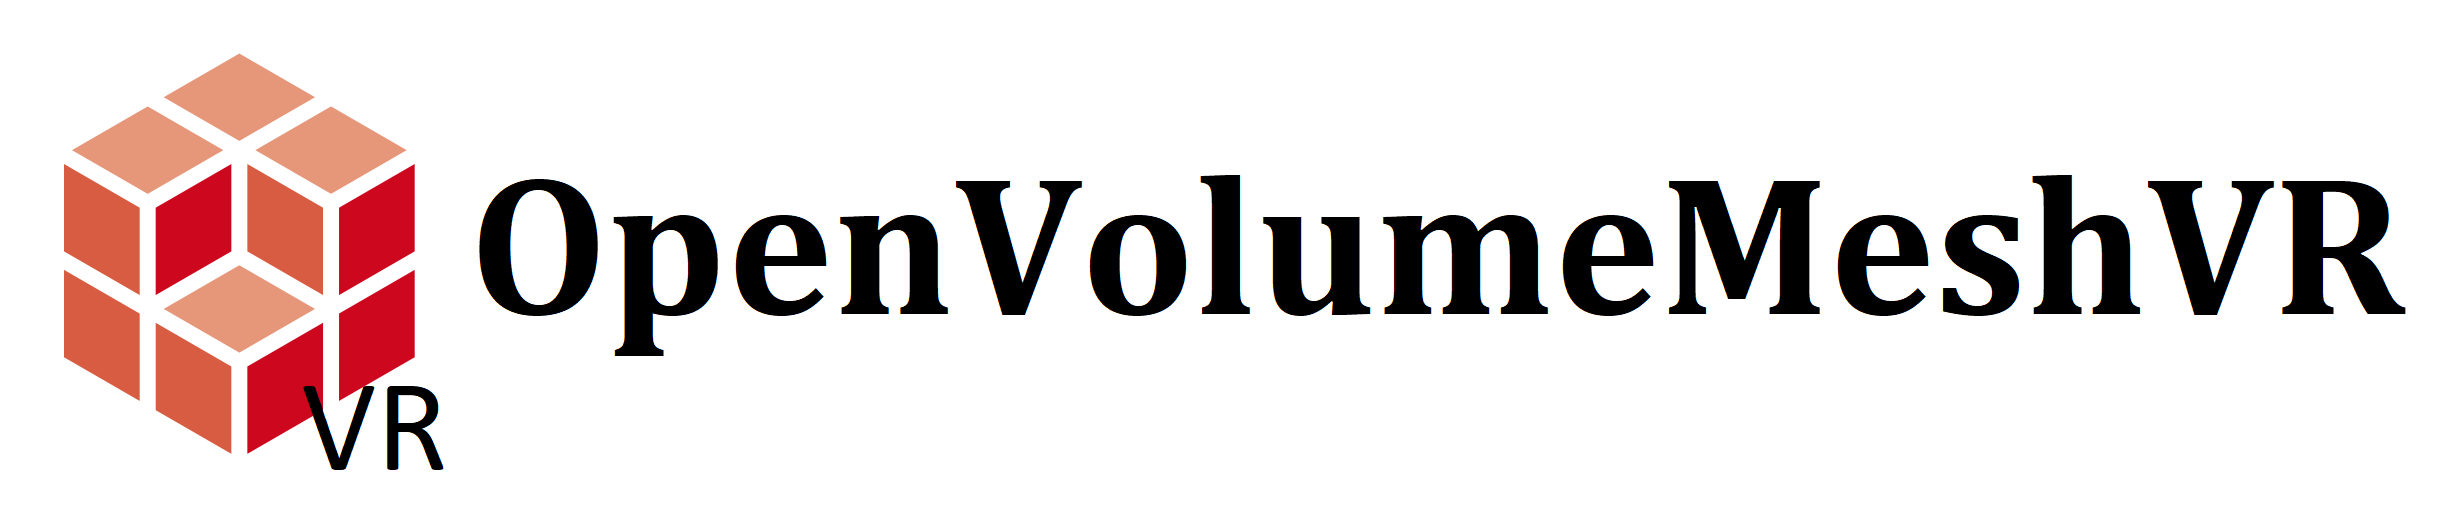
\includegraphics[width=0.75\textwidth]{OpenVolumeMeshVR.png}\par 
	\vspace{2cm}
	{\Large\itshape by Marcel Zauder\par}
	\vfill
	supervised by\par
	Prof. Dr. David \textsc{Bommes}
\end{titlepage}

\begin{abstract}
	\textit{Virtual Reality technology experienced a boom in the last ten years and many different kinds of programs emerged that can be used in the virtual environment. Especially for sketching and drawing this kind of software is well perceived. OpenVolumeMeshVR is such a Virtual Reality mesh sketching application to have a utility for OpenVolumeMesh structures to be designed. The user is enabled to generate simple OpenVolumeMesh structures which also can be modified and viewed. During the development of OVMVR a study for how intuitively a certain approach of controlling a VR application is performed, using already existing software as a reference, and the findings are incorporated in the final application. Additionally, an algorithm for finding cells within a given mesh structure is integrated along with other features.}
	
	\keywords{Virtual Reality, Unreal Engine, OpenVolumeMesh, Volume Mesh Sketching}
\end{abstract}

\tableofcontents

\chapter{Introduction}
	Virtual Reality (VR) is one of the most up-and-coming technology sectors in informatics and is already today a very important component in many different application areas. However, the search term "virtual reality" gives nearly 1'390'000'000 hits (\today). Also in the media VR covers more and more broadcasting time and therefore its acknowledgment is rapidly increasing.  Due to these many people nowadays know the term VR, but barely more than superficially and only a few of them have ever ventured into virtual reality. Even in modern companies, such as architecture bureaus and the automobile industry, VR is used to create 3D models of prototypes so it can be shown to investors or to highlight problems or hints to make the product better. However, the biggest application of VR is in the gaming industry, in which this type of control is very well received. Therefore, it is not surprising that many companies are dealing with this area to further develop this technology.	
	
	\section{Methodology}
	\startsection
		In this bachelor thesis, a brief overview of volume sketching in VR is given and how it is used today. Especially highlighted is the usage of it in terms of the creation of 3D meshes. Considering this, already published programs from Google and Microsoft are inspected and their pros and cons are determined by executing a survey about intuitiveness and usability. Also, the used Unreal Engine 4 and OpenVolumeMesh are introduced and presented.
	\closesection
	
	\section{Motivation and Goal}
	\startsection
		OpenVolumeMesh is a data structure that can represent heterogeneous 3-dimensional polytopal cell complexes (\citep{KBK13}, Section \ref{OpenVolumeMesh}). Until the start of this bachelor thesis, to create a new OpenVolumeMesh mesh, it either is converted from an already existing 3D volume mesh or must be generated by coding. Also, the viewing of individual meshes was very difficult to achieve due to OpenVolumeMesh and OpenFlipper not having a particularly good renderer. \\
		Therefore the goal of this bachelor thesis is to create an application that is capable of generating and modifying simple OVM meshes and also loading and viewing these within a virtual environment. This application can both be used with a "Virtual Reality Head-Mounted Display" or with the use of a mouse and keyboard on a desktop computer. This application will be implemented with the use of the Unreal Engine. It is a C++-based game engine that was advantageous to the integration of OpenVolumeMesh because its source code is also written in C++. 
	\closesection
	
	\section{Limitations}
	\startsection
		Because the goal of this bachelor thesis is to develop an application with which it is possible to create simple meshes based on the OpenVolumeMesh data structure, the program will not be able to display meshes with an entity number greater than 5'000. A higher number of entities can be reached if for example the engine's settings themselves are overwritten, like culling, render distance or the display entities are altered to simpler structures. In the end, this will only increase the limit to a maximum of 2'162'688 objects because this is the limit set by the Unreal Engine itself. \\
		Unfortunately due to the Covid-19 pandemic and the associated inaccessibility of the VR equipment the Virtual Reality implementation is not as refined as possible and does lack in terms of bug safeness and working features. However, during this bachelor thesis, the ability to use this program with a mouse and keyboard was implemented, which is working as intended.
	\closesection
	

\chapter{Research}

	\section{Volume Sketching in Virtual Reality}
	\startsection
		One of the first applications for creating a 3D object with so-called tangible tools was developed in 2001 by Steven Schkolne, Michael Prutt, and Peter Schröder called \textit{Surface Drawing} \cite{SurfaceDrawing}. This tool is intended to combine the step of artists needing to sketch with pen and paper before the actual creation of the 3D shapes with B-spline patches. Hence, the actual creation was done on the sketchpad whereas the computer was only used to specify the previously generated objects. The tool uses the Responsive Workbench, created by W. Krüger and B. Fröhlich, as a semi-immersive environment. This actual workbench tracks the position and movement of different tools and the hand. For each task in the creation of 3D shapes a different tool is used, i.e. tongs to modify the object or a squeezable eraser. The computer-generated objects are then displayed on Augmented-Reality glasses or are directly projected onto the workbench itself. \\
		A year later, Michele Fiorentino et al. developed the \textit{Spacedesign} application \cite{SpaceDesign}. Similar to \textit{Surface Drawing} it uses AR-glasses, in particular the Sony Glasstrom displays, to project the virtual environment. The user is controlling the application with a pen that is connected to the computer. Its position and movement are tracked and based on these variables a 3D sketch is computed. Different from the previously mentioned program \textit{Spacedesign} already uses wireless tangible tools to allow more freedom while being in the virtual environment. \\
		Following the high success of the VR devices from HTC and Oculus, Machuca et al. established the tool \textit{Multiplanes} in 2017 \cite{Multiplanes}. The problem they saw in former applications was that they were built on the freehand drawing technique. This approach though being a very intuitive and effective method for generating 3D sketches is most often not the desired result. The handsfree drawing is "beautified" by suggesting the most probable shape that the user wanted to create. This "beautification" step takes into consideration the previously made strokes as well as geometrical relationships. Another important point in the development was the ease of use of the application, as extensive training was undesirable for the authors. \\
		With the boom in interest in VR, more software emerged, and in 2018 Eroglu et al. commenced the development of \textit{Fluid Sketching} \cite{FluidSketching}. The focus of this application is to use strokes that behave like fluids, which can differ in viscosity or trailing entities, in order to create art that in reality requires many hours of preparation and high levels of expertise and training. Additionally, it allows the use of thermodynamic properties such that the different fluids diffuse over time resulting in a natural behavior of the components.
	\closesection
	
	\section{Provided Software} \label{Provided Software}
	\startsection
		In the following section, a collection of 3D graphic software is presented and examined. In each of those applications, it is possible to create 3D structures some rather on an architectural level some on an artistic level like drawing or modeling. Also, the implementation of equal tools or the approach to the same task sometimes differs on a high basis. \\
		Ideas and suggestions, which are drawn from these, then form the foundation of the program developed during the bachelor thesis.
		\subsection[Google Blocks]{Google Blocks \textsc{\small{\cite{GB4}}}}
		\startsubsection
			Google Blocks is, compared to the other applications listed here, not a comprehensive but a very easy-to-use program. There are 6 main features at the moment: placement of ready-made 3D objects, drawing freehand lines, coloring, modifying, moving, and deleting objects and structures. Within each of these exist also subfunctions, such as grouping, copying, and scaling up or down, available. The resulting scenes can then be exported as a .obj file or as an animated gif. Google Blocks also has its own marketplace, where creations of other users can be viewed and imported as well as own structures can be uploaded and published.
		\closesection
		\subsection[Google Tilt Brush]{Google Tilt Brush \textsc{\small{\cite{GTB}}}}
		\startsubsection
			Google Tilt Brush offers the possibility to draw and paint in VR. Unlike the other software, here the artistic aspect and not the creation of volumetric meshes or 3D structures is at the point of interest. Therefore a work of art can be created with many different types of "dynamic brushes". A big variation provides the virtual palette which includes oil, ink, and watercolors besides paints with effects as fire, glow, and smoke. Although it is possible to incorporate shapes into the scenery, this option is of less importance. \\
			For executing showcases to a group of observant in-game cameras can be placed, so creations can be viewed from different perspectives and not only in first-person.
		\closesection
		\subsection[Masterpiece VR]{Masterpiece VR \textsc{\small{\cite{MVR}}}}
		\startsubsection
			In Masterpiece VR 3D  sculptures can be modeled by using "virtual clay". It is mainly used to create characters, objects, and asset visuals which then can be exported to Unity or Marmoset. It is also possible to create intricate objects due to the implementation of "pinch" and "noise" tools which roughen the surface of the clay sculptures. In addition, the environment can be manipulated so each creation can be viewed under different light conditions and in various settings. \\
			Furthermore, Masterpiece VR can invite other collaborators and spectators to experience VR modeling in multiplayer.
		\closesection
		\subsection[Microsoft Maquette]{Microsoft Maquette \textsc{\small{\cite{MSM}}}}
		\startsubsection
			Microsoft Maquette is one of the more feature-heavy applications tested within the scope of this bachelor thesis. Primarily, it is used to quickly create spatial prototypes which can then be used in other applications like in the Game Engine Unity for (environmental) assets. Finished objects can be saved in an "inventory"-like menu tab and easily accessed and multiplied within Maquette itself making it much easier to create repeating patterns. It is also possible to place text fields and generate 3D texts within the virtual space to create 3D assets which can then be placed in videogames for example. Because the content which is generated with Microsoft Maquette can be exported in many different file types, like .fbx, .glb, and .gltf, these objects can then be viewed and used in many different applications like Blender or the Unity game engine. \\
			Since November 2021 Microsoft does not actively develop this application any more and used the feedback that was gathered during the Beta phase to be applied in future Mixed Reality applications.
		\closesection
	\closesection
			
	\section[Unreal Engine 4]{Unreal Engine 4 \textsc{\small{\cite{UE4}}}}
	\startsection
		Unreal Engine 4 (UE4) is the latest version of the game engine developed by Epic Games. The first version of Unreal Engine appeared together with the FPS game Unreal in 1998 established by Tim Sweeney, the founder of said company. Due to being written in C++ and also being source-available since 2014 it can be implemented and imported very easily on many different platforms. By already supporting a huge amount of these platforms, it is a highly used engine for programming and setting up a multitude of various games. \\
		The framework consists of a graphic engine and its related script language UnrealScript among many other things. Also, UnrealEd, a level editor, is provided with which the layout of maps and levels are changeable on the fly. With its possibility of blueprint visual scripting even complex prototypes can be integrated into the virtual world without needing a high acknowledgment of coding. This makes Unreal Engine even more suitable for the average programmer. By visualizing the different behaviors and dependencies the debugging is also quite easy. \\
		Due to the multiplayer experience frequently being used, UE4 adds a scalable server/client architecture to get the ability to implement this component. Additionally, Unreal Engine has gathered a huge community behind itself which means that many different tools and feature integrations can already be downloaded and used via GitHub or the Marketplace. \\
		Through close collaboration between Epic Games and the world's leading hardware and software manufacturers, UE4 is also geared towards the use of Virtual Reality (VR), Augmented Reality (AR), and Mixed Reality (MR) and therefore continues to evolve and improve in these areas.
	\closesection

	\section[OpenVolumeMesh]{OpenVolumeMesh \textsc{\small{\cite{OVM}}}} \label{OpenVolumeMesh}
	\startsection
		OpenVolumeMesh (OVM) is a generic data structure based on OpenMesh in order to handle arbitrary polyhedral meshes developed by M. Kremer, D. Bommes, and L. Kobbelt in 2013. It uses the idea of half-edges and accordingly creates half-faces of different orientations (Figure \ref{HalfedgeHalfface}). The biggest advantage of OVM, however, is that the data structure is equivalent to an indexed array, allowing access to run in constant time complexity.
		\begin{figure}[H]
			\begin{center}
				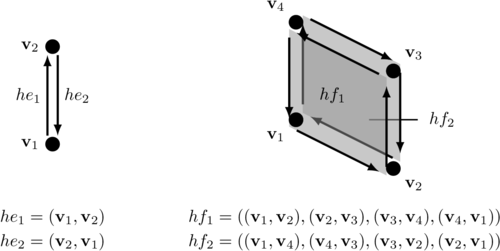
\includegraphics[width=0.5\textwidth]{halfedge_halfface.png} 
				\caption{Illustration of Halfedge and Halfface}
				\label{HalfedgeHalfface}
			\end{center}
		\end{figure}
		\noindent An edge within a mesh is split up into two half-edges from which each contains a start and an end vertex. Several of these half-edges arranged in a loop make up a half-face. The frontside of a half-face is defined to be the side from which the incidents of all half-edges are directed in a counter-clockwise orientation. Hence, also each face is made up of two half-faces. Furthermore, cells can be acquired by aggregating the half-faces, such that all normals of these are pointing towards the center of the cell. \\
		These entities are the components with which a polyhedral mesh can be defined. A polyhedron is a 3D object that consists of multiple flat polygons. With the use of OVM these polyhedra are most often equivalent to the cells that are defined within a mesh. \\
		Another possibility in OVM is to give each entity multiple dynamic properties of any type. In the resulting application OVMVR, these properties are used to link each entity handle - handles are the instances of the actual item like vertex, edge, etc. - against the representation instances in the virtual world. The actual use of properties like attaching a value that represents a force or some other kind of energy influencing the mesh is not used in this project.
	\closesection

\chapter{Intuition Study}
	
	\section{Concept and Execution}	
	\startsection				
		To decide which specifications the new program should include and how they should be implemented, a test was performed in which two of the given programs, Google Blocks, and Microsoft Maquette, were compared against each other and their intuitiveness was determined. Test worlds for Google Blocks as well as for Microsoft Maquette were created conducive to identifying the advantages and disadvantages of the individual features and to achieve the best possible implementation of the respective functionality. Within these test worlds, the user was faced with different tasks that should be accomplished, i.e. recreating the object the author has placed. The set of tasks consisted of the following:
		\begin{enumerate}[-]
			\item Moving through the virtual environment
			\item generating any object
			\item delete objects
			\item placing pre-made objects (spheres, cubes, etc.)
			\item place objects with the snapping and align feature
			\item color the objects
			\item copy and paste, move, scale and group objects
			\item modify (extruding, subdividing, etc) predefined objects
		\end{enumerate}		
		The tasks between these testing areas were kept as similar as possible so the measurement of the discrepancy of those two programs and their components is representative. In order to rule out that a program benefits by being tested secondarily, and thus previously learned could distort the test results, the process is always varied, so that half of the probands will start with Google Blocks and the other half with Microsoft Maquette. \\
		While the test persons are completing the tasks, notes are taken by the author wherein the intuitiveness of each service is checked according to how fast the functionality is discovered and understood as well as occurring problems are highlighted. At the end of this process an evaluation sheet, which contains questions about how intuitive and simple the different tasks were and which of the programs they preferred, is filled in (Appendix \ref{appendix:questionnaire}).
	\closesection

	\section{Tables}
	\startsection	
		In the following tables, the results of the tests are listed. The scale for the movement part has been chosen differently (1-6), as it focuses on a more specific view to be able to study this functionality very closely and to determine what is perceived as a rather better type of movement. Concerning the other parts, the point of interest was set on which program implemented each particular mode better. For illustrational purposes, the value of 1 has been assigned to the selected option. \\
		In the end, the average value for each component was computed, so the usability and intuitiveness can be easily evaluated. \\		
		\begin{table}[H]
			\begin{center}
			\begin{tabular}{@{}|lll|llllllllllllll|r|@{}}
				\hline
				\multicolumn{3}{|l|}{\textbf{\underline{General}}} & & & & & & & & & & & & & & & \textbf{average $\emptyset$} \\ \hline
				& \multicolumn{2}{l|}{\textbf{Impression}} & \multicolumn{14}{c|}{\small{What application was perceived as the better}} &\\ \hline
				& & Google Blocks & 1 & 0 & 1 & 1 & 1 & 1 & 0 & 1 & 0 & 1 & 1 & 0 & 0 & 0 & 0.57 \\
				& & Microsoft Maquette & 1 & 1 & 0 & 0 & 0 & 0 & 1 & 0 & 1 & 0 & 0 & 1 & 1 & 1 & 0.50 \\ \hline
				
				& \multicolumn{2}{l|}{\textbf{Simplicity}} & & & & & & & & & & & & & & &\\ \hline
				& & Google Blocks & 1 & 1 & 1 & 1 & 1 & 1 & 1 & 1 & 1 & 1 & 1 & 1 & 1 & 0 & 0.93 \\
				& & Microsoft Maquette & 0 & 0 & 0 & 1 & 0 & 0 & 0 & 0 & 0 & 0 & 0 & 0 & 0 & 1 & 0.13 \\ \hline
			\end{tabular}
			\caption{General Evaluation}
			\label{tab:GeneralEvaluation}
			\end{center}
		\end{table}
		
		\begin{table}[H]
			\begin{center}		
			\begin{tabular}{@{}|lll|llllllllllllll|r|@{}}
				\hline
				\multicolumn{3}{|l|}{\textbf{\underline{Movement}}} & & & & & & & & & & & & & & & \textbf{average $\emptyset$} \\ \hline
				& \multicolumn{2}{l|}{\textbf{Intuitiveness}} & & & & & & & & & & & & & & &\\ \hline
				& & Google Blocks & 3 & 2 & 6 & 6 & 3 & 5 & 4 & 4 & 5 & 5 & 5 & 4 & 6 & 4 & 4.43 \\
				& & Microsoft Maquette & 3 & 2 & 5 & 4 & 2 & 4 & 4 & 2 & 4 & 1 & 3 & 5 & 5 & 3 & 3.36 \\ \hline
				
				& \multicolumn{2}{l|}{\textbf{Impression}} & \multicolumn{14}{c|}{\small{How well was the form of movement perceived}} &\\ \hline
				& & Google Blocks & 4 & 1 & 6 & 5 & 6 & 5 & 3 & 5 & 5 & 5 & 5 & 4 & 5 & 4 & 4.50 \\
				& & Microsoft Maquette & 5 & 1 & 5 & 4 & 4 & 4 & 3 & 2 & 5 & 2 & 4 & 5 & 6 & 5 & 3.93 \\ \hline
			\end{tabular}	
			\caption{Movement Evaluation}
			\label{tab:MovementEvaluation}
			\end{center}	
		\end{table}
		
		\begin{table}[H]
			\begin{center}
			\begin{tabular}{@{}|lll|llllllllllllll|r|@{}}
				\hline
				\multicolumn{3}{|l|}{\textbf{\underline{Object Interaction}}} & & & & & & & & & & & & & & & \textbf{average $\emptyset$} \\ \hline
				& \multicolumn{2}{l|}{\textbf{Placing}} & & & & & & & & & & & & & & &\\ \hline
				& & Google Blocks & 1 & 0 & 1 & 1 & 1 & 1 & 0 & 1 & 0 & 1 & 1 & 1 & 1 & 1 & 0.79 \\
				& & Microsoft Maquette & 1 & 1 & 0 & 1 & 0 & 0 & 1 & 0 & 1 & 0 & 0 & 0 & 0 & 0 & 0.36 \\ \hline
				
				& \multicolumn{2}{l|}{\textbf{Moving}} & \multicolumn{14}{c|}{\small{only Google Blocks implemented an explicit mode}} &\\ \hline
				& & Google Blocks & 1 & 0 & 1 & 1 & 1 & 1 & 1 & 1 & 1 & 1 & 1 & 0 & 1 & 1 & 0.86 \\
				& & Microsoft Maquette & 1 & 1 & 0 & 0 & 0 & 1 & 0 & 0 & 0 & 0 & 0 & 1 & 0 & 0 & 0.29 \\ \hline
				
				& \multicolumn{2}{l|}{\textbf{Snapping}} & & & & & & & & & & & & & & &\\ \hline
				& & Google Blocks & 0 & 0 & 1 & 1 & 1 & 1 & 1 & 1 & 1 & 1 & 1 & 1 & 0 & 0 & 0.71 \\
				& & Microsoft Maquette & 1 & 1 & 0 & 1& 0 & 0 & 0 & 0 & 0 & 0 & 0 & 1 & 1 & 1 & 0.43 \\ \hline
				
				& \multicolumn{2}{l|}{\textbf{Deleting}} & & & & & & & & & & & & & & &\\ \hline
				& & Google Blocks & 1 & 0 & 1 & 1 & 0 & 1 & 1 & 1 & 1 & 1 & 1 & 0 & 0 & 0 & 0.64 \\
				& & Microsoft Maquette & 1 & 1 & 0 & 1 & 1 & 0 & 1 & 0 & 1 & 0 & 1 & 1 & 1& 1 & 0.71\\ \hline
				
				& \multicolumn{2}{l|}{\textbf{Coloring}} & & & & & & & & & & & & & & &\\ \hline
				& & Google Blocks & 1 & 0 & 0 & 1 & 1 & 1 & 0 & 0 & 0 & 1 & 1 & 0 & 0 & 0 & 0.43 \\
				& & Microsoft Maquette & 0 & 1 & 1 & 1 & 1 & 0 & 1 & 1 & 1 & 0 & 0 & 1 & 1 & 1 & 0.71 \\ \hline
				
				& \multicolumn{2}{l|}{\textbf{Modifying}} & \multicolumn{14}{c|}{\small{only Google Blocks implemented an explicit mode}} &\\ \hline
				& & Google Blocks & 1 & 1 & 1 & 1 & 1 & 1 & 1 & 0 & 0 & 1 & 1 & 0 & 1 & 1 & 0.79\\
				& & Microsoft Maquette & 1 & 0 & 0 & 1 & 0 & 0 & 0 & 1 & 1 & 0 & 0 & 1 & 0 & 1 & 0.43 \\ \hline

				& \multicolumn{2}{l|}{\textbf{Grouping}} & \multicolumn{14}{c|}{\small{only Microsoft Maquette implemented an explicit mode}} &\\ \hline
				& & Google Blocks & 1 & 1 & 0 & 0 & 0 & 0& 1 & 1 & 1 & 0 & 0 & 1 & 0 & 0 & 0.43 \\
				& & Microsoft Maquette & 1 & 0 & 1 & 1 & 1 & 1 & 0 & 0 & 0 & 1 & 1 & 0 & 1 & 1 & 0.64 \\ \hline				
				
				& \multicolumn{2}{l|}{\textbf{Copying}} & \multicolumn{14}{c|}{\small{only Microsoft Maquette implemented an explicit mode}} &\\ \hline
				& & Google Blocks & 0 & 1 & 0 & 1 & 0 & 1 & 1 & 1 & 0 & 0 & 0 & 1 & 0 & 0 & 0.43 \\
				& & Microsoft Maquette & 1 & 0 & 1 & 1 & 1 & 0 & 1 & 0 & 1 & 1 & 1 & 0 & 1 & 1 & 0.71 \\ \hline
			\end{tabular}
			\caption{Object-Interaction Evaluation}
			\label{tab:InteractionEvaluation}
			\end{center}				
		\end{table}
		
		\begin{table}[H]
			\begin{center}
			\begin{tabular}{@{}|lll|llllllllllllll|r|@{}}
				\hline
				\multicolumn{3}{|l|}{\textbf{\underline{Interface}}} & & & & & & & & & & & & & & & \textbf{average $\emptyset$} \\ \hline
				& & Google Blocks & 0 & 0 & 1 & 1 & 1 & 1 & 0 & 1 & 0 & 1 & 1 & 0 & 1 & 0 & 0.57 \\
				& & Microsoft Maquette & 1 & 1 & 0 & 0 & 0 & 0 & 1 & 0 & 1 & 0 & 1 & 1 & 1 & 1 & 0.57 \\ \hline
			\end{tabular}
			\caption{Interface Evaluation}
			\label{tab:InterfaceEvaluation}
			\end{center}
		\end{table}
	\closesection
			
	\section{Results and Evaluation}
	\startsection
		\vspace{0.1cm}
		\subsection{Impression and Layout}
		\startsubsection
			In general neither program is significantly better or worse, nevertheless, a few discrepancies can be recognized between some functionalities. The main difference is within the simplicity because Google Blocks has much fewer editing tools than Microsoft Maquette and is therefore considerably more surveyable and incomplex (referring Table \ref{tab:GeneralEvaluation}). \\
			Concerning the most interesting point, changing the in-game position, the survey shows, that Google Blocks is slightly easier to understand and to work with. However, moving through the world using the "swimming" concept of Maquette is not considered the best way to implement this essential part (referring to Table \ref{tab:MovementEvaluation}). Besides moving through the entire world using that concept often lead to motion sickness, because the brain assumes to move through space without actually moving the body. A huge problem for both designs is that the "Grab" buttons, which are located on each side of both controllers, are difficult to use and not very handy. Therefore, these should only be used sporadically. \\
			In terms of the interface and selection menu, none of these programs is especially better or worse than the other one (referring to Table \ref{tab:InterfaceEvaluation}). Nevertheless, it has been observed that the graphical display of the menu, which is located on the side of one controller, has often restricted and reduced the working area. To prevent this, it would be appropriate to implement a hiding option or place it so that it does not interfere with the user. A good example is Google Tilt Brush, where the selection menu is located above the controller.
		\closesection
		\subsection[Object Interaction]{Object Interaction \small{\texttt{(referring Table \ref{tab:InteractionEvaluation})}}}
		\startsubsection
			A general overview of the object interaction statistics suggests by implementing an explicit mode the associated tasks were perceived as much more pleasant and easier to use. This is also reflected in the fact that when one program had implemented a corresponding mode, whereas the other did not, that program was most likely to be considered more intuitive in that particular area. Therefore, this leads to the conclusion that for each interaction a demarcating mode should be implemented in order to ensure a high degree of user-friendliness. \\
			Placing given objects and shapes is quite similar in both tested programs, whereas generating freehand lines is much easier in Microsoft Maquette because a more meaningful signifier is used. But in the study, Google Blocks received a better rating. A reason for this is a much smaller, and therefore clearer, collection of given objects. Also switching between the different objects is easier in Google Blocks by swiping through using the touchpad. In Microsoft Maquette on the other hand every shape must be selected individually from the selection menu which is more inconvenient and time-consuming. \\
			For moving objects Google Blocks implemented a specific "Grabbing"-mode so it was easier for the probands to figure out how to manipulate the position of structures. On the other hand, Microsoft Maquette uses the "Grab"-buttons which intuitively makes sense because users are actually grabbing the thing. However, since the "Grab"-buttons are difficult to handle, the useability of this feature was considered rather bad. Therefore Google Blocks performed much better in that section and a significantly larger number of subjects considered it more pleasant. \\
			The applications include two different methods for implementing rotational snapping and alignment. In Google Blocks the left-handed trigger must be kept pressed, whereas, in contrast, Microsoft Maquette uses an additional button on the right-handed touchpad to toggle this mode on and off. The study found that the former was more comfortable to use, as the user did not need to check whether the mode is toggled on or off. \\
			There are two different variants for deleting objects in both software: On the one hand, an independent mode is implemented, on the other hand, the object can be thrown away so it disappears. Especially the "Disposal"-option was considered very intuitive and useful. Since this feature is much easier to apply and more reliable in Microsoft Maquette than Google Blocks, it was slightly better rated. \\
			Coloring in Google Blocks holds the problem in that the color palette is located on the back of the selection menu and is therefore not directly visible to the user. Consequently, a lot of time was needed to find it, which ultimately harmed the user's opinion of this part. In Maquette the color selection was much more extensive, due to the implementation of an RGB palette. Also, an eyedropper was added, whereby a color selection of already colored objects was possible. However, this involved the problem that the extraction line, which had to be directed onto the object to select the color, was not recognized as such, which made the handling of this option slightly difficult. Nonetheless, Microsoft Maquette did better in this area due to the greater color choice and the more convenient operation. \\
			Exclusively Google Blocks realized an explicit tool for modifying, as subdividing, extruding, and extracting, objects and their assets, while in Microsoft Maquette only the length, width, and depth of a structure are changeable. Also, handling the feature in Maquette, which requires a synchronized movement of both controllers, was not without problems. Accordingly, the test subjects perceived Google Blocks as a much more pleasant and better option for this type of interaction. \\
			For grouping and copying of several structures and objects both software have implemented an associated tool. In Google Blocks, however, this tool is hidden inside the "Grab" feature, which means it is not directly recognized. In contrast, in Microsoft Maquette, there are even several fields, within the copy function, into which object groups can be copied in order to quickly duplicate them. These details ultimately lead to Maquette performing better in the survey for both options, and more test subjects found it easier to use.
		\closesection
		\subsection{Conclusion} \label{IntuitionStudyConclusion}
		\startsubsection
			The survey generally shows that each function is much easier to use if there is a separate, special mode for it. In addition, each of these modes should be clearly described and the functionality easy to recognize and quickly understood. Also, within a mode, not many other specifications should be present, as this leads to a higher degree of complexity of the program. \\
			From the testers' reports and the author's notes, it further emerges that the "Grab"-buttons are very difficult to use, and thus an "over-use" of them is considered negative. On the other hand, the touchpad is acknowledged as a very good control option, so a good implementation of this can lead to a high level of usability. What is also noticeable is that many testers favor haptic feedback as very useful and should therefore be taken into account. \\
			Another problem was that the orientation of the interface menu often severely restricted the workspace. Thus, an implementation as found in Google Tilt Brush with this menu above the secondary controller should be considered. Also, a toggle mode to hide and show the menu can counteract this problem. \\
			Ultimately, this study has produced some ideas for implementing various specifications and has been able to inform about the differences in the usability of the modes.
			\newpage
			\paragraph{Drawn Conclussions for OpenVolumeMeshVR Implementation} \hfill \\
			The most important thing that could be drawn from this intuition study was that for each task or feature the application should provide a separate mode to accomplish it. These different modes should also not be too extensive and not provide any additional features that might not be directly accessible but need a certain keyboard or controller shortcut in order to be used. \\
			Additionally, a toggleable menu will be implemented such that the working space is not restricted or reduced by letting the user decide when it is visible and when it should be hidden. Furthermore, this also gives the advantage that the buttons can be made much larger to ease the selection of the different modes. On the other hand when in the mouse-keyboard control mode a Heads-Up Display has been integrated which shows at all times which modes can be used, with which number-key they can be accessed, and in which mode the user currently is.  \\
			In terms of movement, it was decided that the user can only pass through the virtual environment by actually walking. In order to be able to see the whole object, it was determined that it is a better approach to grab the whole mesh and move it by itself. For the mouse-keyboard control this part does not matter and the usual "WASD"-movement was implemented.			
		\closesection
	\closesection
		
		
\chapter{Documentation OpenVolumeMeshVR}
	OpenVolumeMeshVR is a sketch tool in which simple meshes can be constructed and viewed. Thusly created meshes can then be saved as OpenVolumeMesh files.
	\begin{figure}[H]
		\begin{center}
			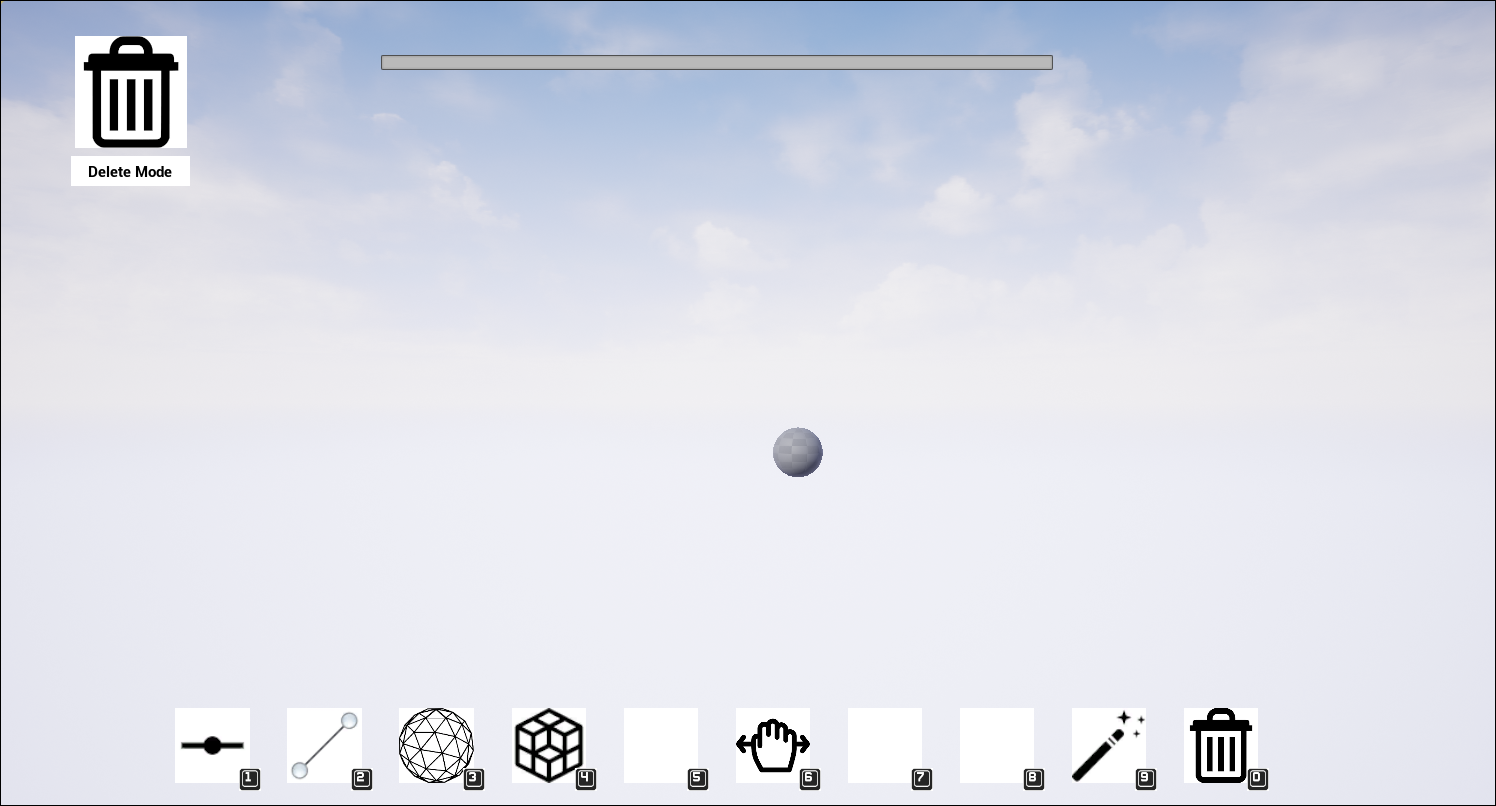
\includegraphics[width=0.95\textwidth]{InGame_Screenshots/FP_View.png}
			\caption{View of OpenVolumeMeshVR using Mouse-Keyboard (MK) Control}
			\label{FPView}
		\end{center}
	\end{figure}
	\noindent The ball which can be seen in the middle of Figure \ref{FPView} will be referred to as the \textsc{PlacementChaperone}. This is the OpenVolumeMeshVR version of the cursor with which the selection, placing, and deletion of the different entities can be performed. The distance of it from the player can be altered by using the mouse wheel. When OpenVolumeMeshVR in VR mode the \textsc{PlacementChaperone} will be part of the right-hand controller. \\
	The player can be moved around by using the WASD-keys and Space/Alt to move up and down when in "MK-Control" or by actually moving around when in "VR-Control". To confirm the placement of an entity or likewise either use the left mouse button or the B-Trigger on the right VR controller. The menu can be entered by either using the Escape or "M" key on the keyboard or the B-trigger of the left VR controller. \\
	In order to generate and modify OVM meshes, different modes have been implemented. On the bottom, the already implemented features are indicated and the associated keys with which the mode can be chosen are displayed.
	\section{Spawning and Placing Entities}
	\startsection
		When placing a vertex a representation of it is spawned in the virtual world and the vertices' position is handed over to the OVM data struct. \\
		Placing an edge can be accomplished in different ways. If no pre-generated vertex is selected a new vertex will be spawned and a preview of the edge can be seen connecting the newly generated vertex with the \textsc{PlacementChaperone}. When a vertex is selected no new vertex will be created. The same is true if the end vertex of the edge is defined so that either a preexisting can be selected or a new one is spawned. The edge is then spawned correctly connecting the start vertex with the end vertex. \\
		When creating a face the same procedure is done as for the placement of an edge, but already existing edges can be included in the face by selecting both start vertex and end vertex. If no edge is between two vertices, regardless of whether they were newly spawned in or not, a new one will be generated. In order to finish the face either the F-button must be pressed or the vertex selected first must be selected a second time, hence spawning a face. The face is not added to the data structure until the placement of it is confirmed. By pressing the right mouse button the selection is discarded and all newly spawned vertices and edges are destroyed.
	\closesection
	
	\section{Finding and Generating Cells}
	\startsection
		For the purpose of creating cells within the mesh a cell finding algorithm has been implemented (for further details refer to section \ref{CellMode}). In order to start the CellFindingAlgorithm, the user has to select a half-face as the starting point, while being in the "CellMode". Because in OVMVR half-faces are not a single component that is shown, but only the face on its own is present, the user is placing the \textsc{PlacementChaperone} on the preferred side of a face, so the direction to which the cell should be created is known to the algorithm, simulating the behavior if a certain half-face would have been selected. If a valid one is found all the faces that are part of the cell are highlighted. By pressing the F-button (button to confirm the selection) the cell is placed, the representation is a 50\% downscaled version of the actual cell, and also added to the OVM data structure. The algorithm will either terminate by highlighting a found cell containing the selected face in red or won't mark anything at all and indicates that it has not found anything currently indicated by an OnScreenDebugMessage.
	\closesection
	
	\section{Moving different Entities}
	\startsection
		In OVMVR it is also possible to modify the positions of vertices, edges, faces, and even cells by moving them around. With the \textsc{PlacementChaperone} the component which should be moved can be selected and the position of the selected component is following the position of the \textsc{PlacementChaperone} until the new position is confirmed or the mode is canceled, in which case the previous position of the component is restored. Based on the new position of the component adjacent, connected entities may also change their position and appearance. These directly affected entities as well as the selected component will be highlighted during the process and a preview is generated every frame.
	\closesection
	
	\section{Delete Entities}
	\startsection
		When deleting an entity of any kind, all other entities that are dependent on the existence of it, like an edge that needs two vertices, will be deleted as well. The dependency graph would look as follows:
		\startsubsection
			Vertex $\rightarrow$ Edge $\rightarrow$ Face $\rightarrow$ Cell
		\closesection
	\closesection
	
	\section{Highlight individual Components}
	\startsection
		When in the "Highlight-Mode" the user can choose between one of three different colored, predefined materials with which the different entities can be colored. The currently chosen material is displayed on the \textsc{PlacementChaperone} and can be changed by clicking the ChangeColor Key (per default key "C"). The highlighted entities will be reset if either the mode is canceled (with the left mouse button) or the user changes to another mode.
	\closesection
	
	\section{Save and Load OVM Files}
	\startsection
		It is possible in OVMVR to save the generated mesh as an OVM file in order to use it in OpenFlipper for example or using the BlenderInterrup tool creating a Blender file so that it can be viewed in the Blender application. Already predefined OVM files can be loaded into OVMVR so they can be viewed and modified. The current limitation is 5'000 entities because otherwise, the loading can take a very long time or the application can crash if too many vertices and edges must be displayed. Additionally, when loading an OVM file the user can increase or decrease the bounding box by inserting the desired diagonal bounding box length into the input box next to the load button. It was integrated additionally that no letters but only numbers can be used as an input in that field.
		\begin{figure}[H]
			\begin{center}
				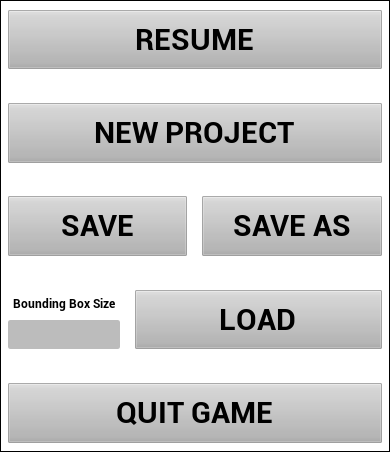
\includegraphics[width=0.35\textwidth]{InGame_Screenshots/FP_PauseMenu.png}
				\caption{Pause Menu}
			\end{center}
		\end{figure}
		\noindent If this input is either equal to zero or empty the bounding box size will be set to a predefined value. This increase of the bounding box will also affect the later saved object because the positions of the vertices themselves are altered.
	\closesection
	
	
\chapter{Implementation}

	\section{Project Structure}
	\begin{tabular}{@{}p{0.65\textwidth}p{0.3\textwidth}@{}}
		\begin{tabular}{p{0.63\textwidth}}
			OpenVolumeMeshVR is a C++ Unreal Engine project which means that additionally to the Unreal Engine's blueprint approach to programming an application native C++ files are integrated into it. As can be seen in Figure \ref{UE4Blueprint} from the native C++ files an Unreal Engine Blueprint can be created. These Blueprints are then used to create the In-Game Instances which are part of the application's environment. The advantage of using this approach is that the developer can implement the much more code-intensive functionalities within the C++ file and then use the Blueprint Class to add further functionalities, like input handling or displaying the HUD and pause menu using UE's Visual Code. Furthermore, when wanting to spawn many instances of a certain class, with for example the component representations (see Section \ref{ComponentRepresentation}), an Actor Blueprint based on the associated C++ class can be created and then can be easily spawned into the world.
			\begin{figure}[H]
				\begin{tikzpicture}
					% Start Point
					\coordinate (start) at (0,0);
						
					% Different Icons
					\node[right=0.75cm of start] (CPPFile) {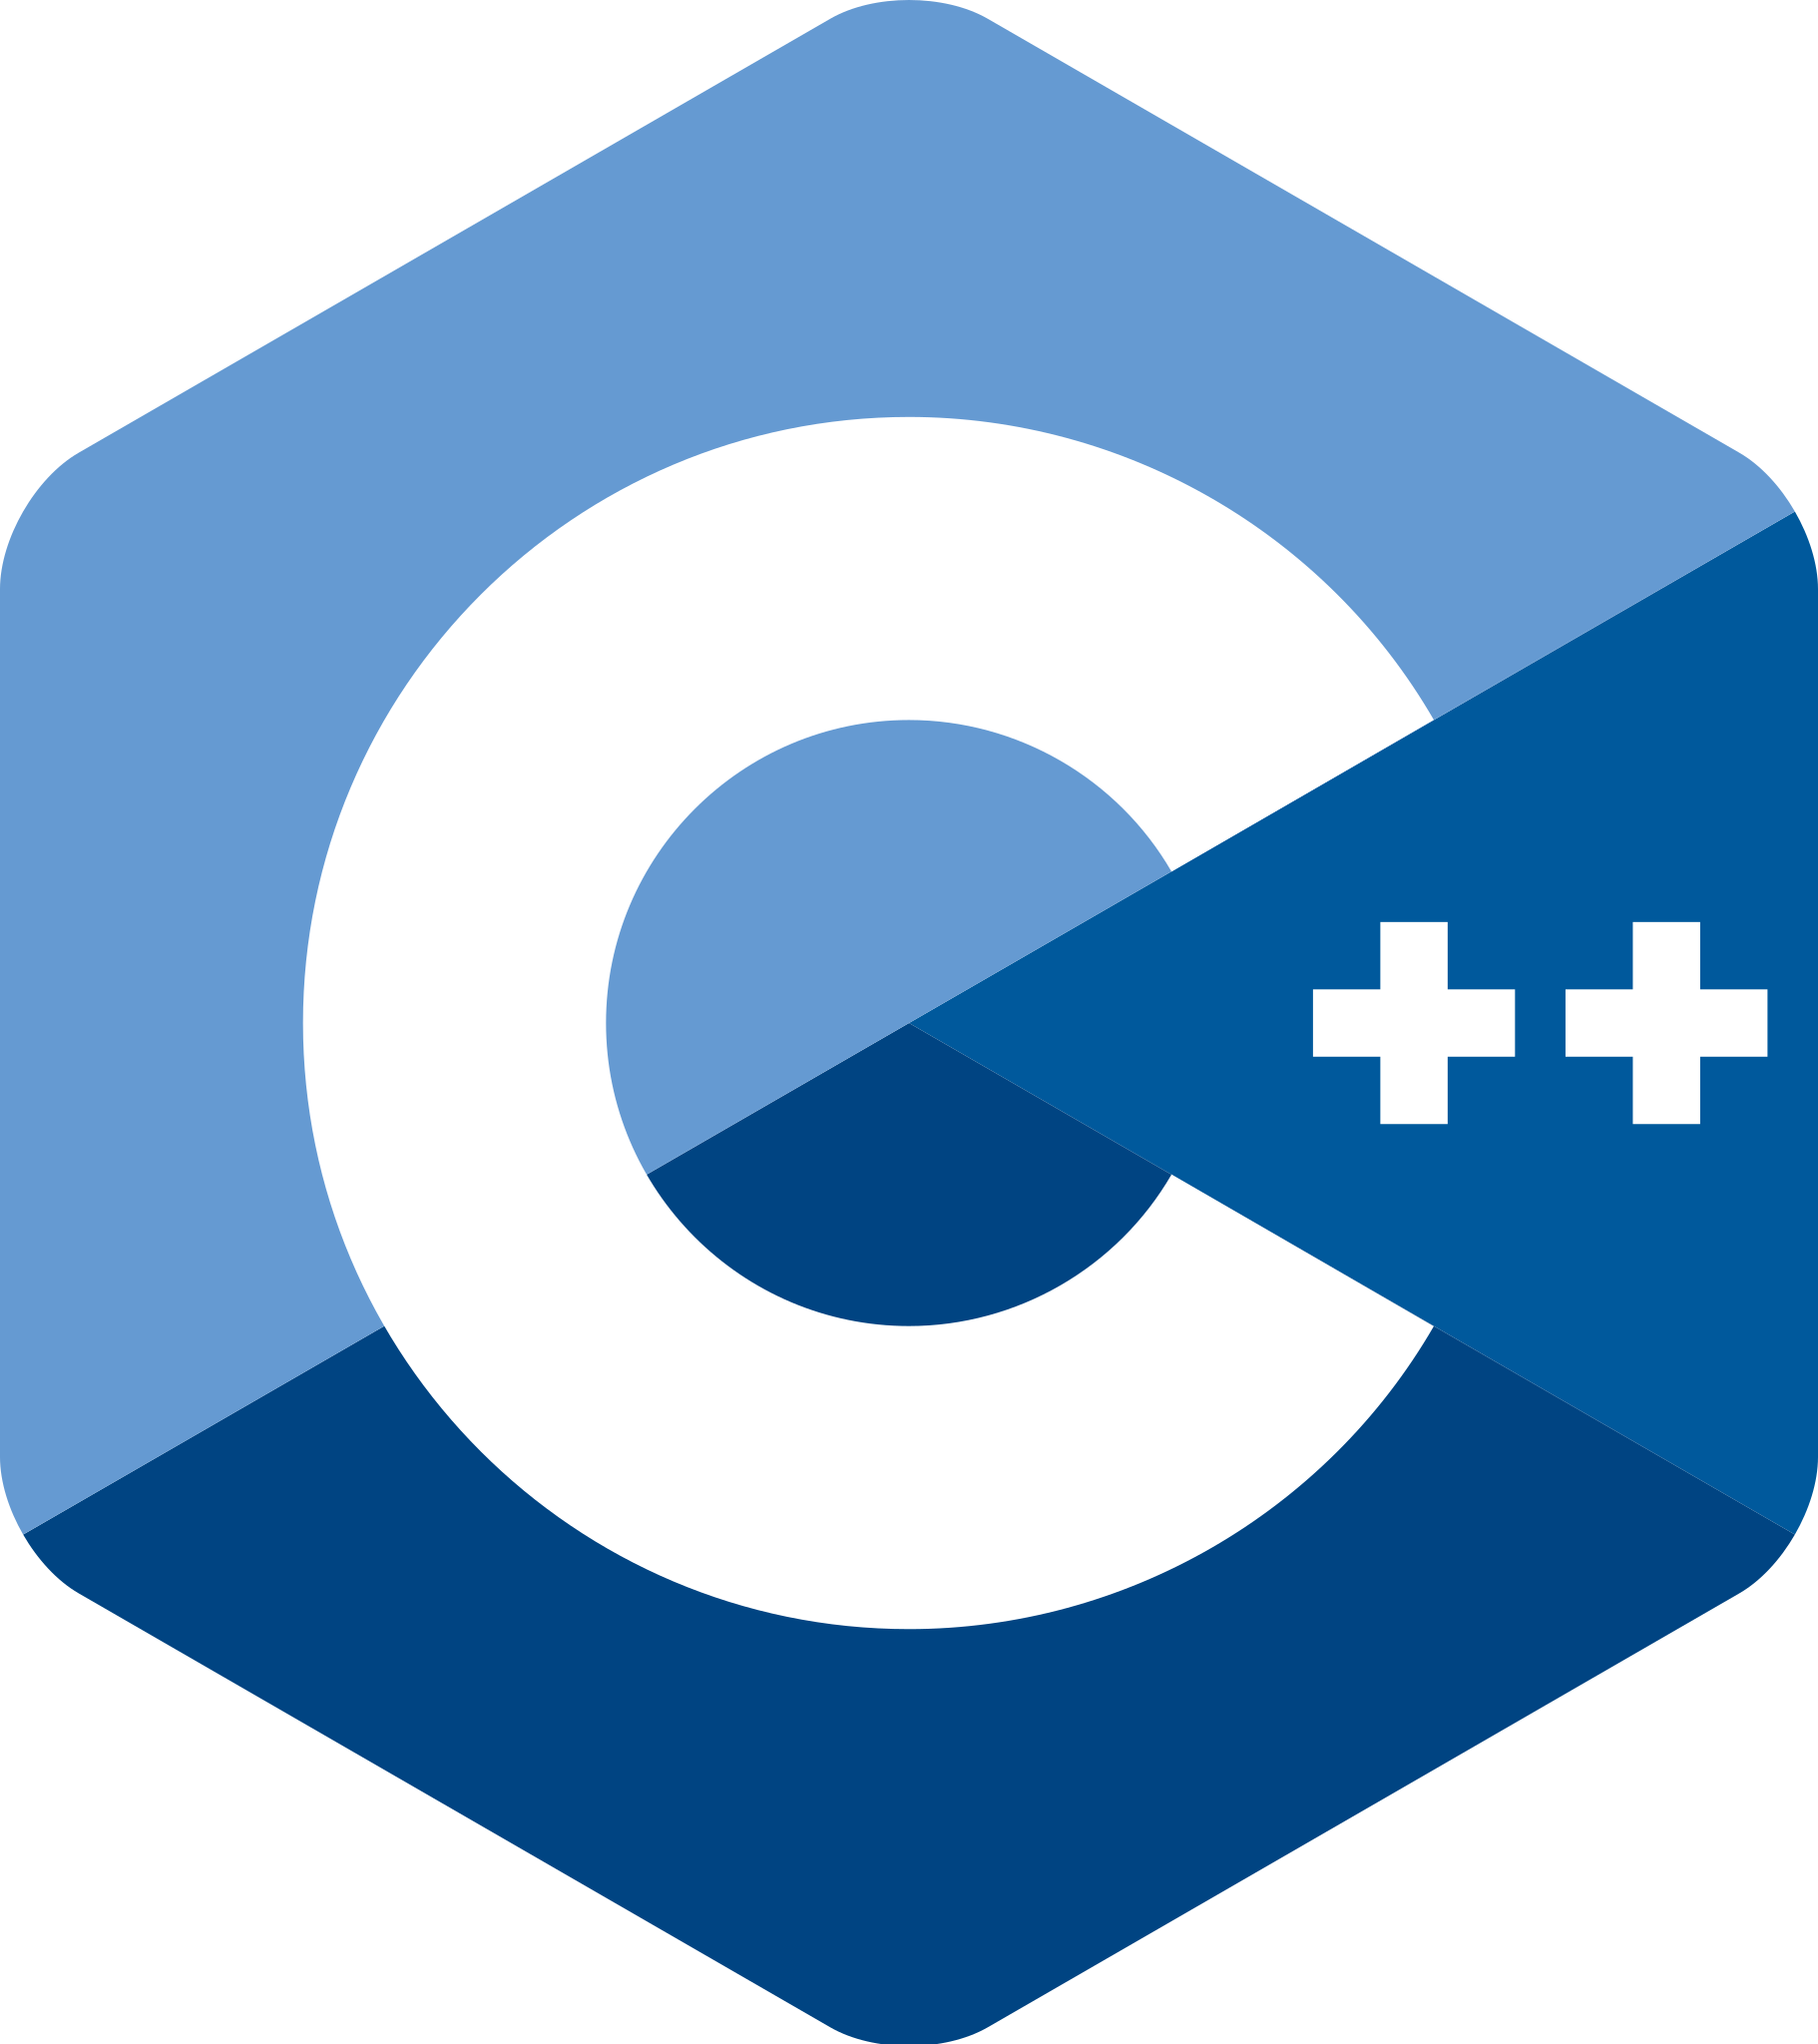
\includegraphics[width=0.1\textwidth]{Blueprint_Explanation/CPP_Icon.png}};
					
					\node[right=2cm of CPPFile] (Blueprint) {
\includegraphics[width=0.1\textwidth]{Blueprint_Explanation/Blueprint_Icon.png}};
					
					\node[right=2.5cm of Blueprint] (Actor) {
\includegraphics[width=0.075\textwidth]{Blueprint_Explanation/Actor_Icon.png}};
					\node[above=1pt of Actor] (Pawn) {
\includegraphics[width=0.075\textwidth]{Blueprint_Explanation/Pawn_Icon.png}};
					\node[below=1pt of Actor] (Hud) {
\includegraphics[width=0.075\textwidth]{Blueprint_Explanation/HUD_Icon.png}};
					
					% Captions
					\node[below=0.1cm of CPPFile] (CAP:CPPFile) {C++-File};
					\node[below=0.1cm of Blueprint] (CAP:Blueprint) {Blueprint};
					\node[below=0.1cm of Hud] (CAP:CPPInstance) {In-Game Instances};
					
					% Arrows
					\draw[->] (CPPFile) edge (Blueprint);
					\draw[->] (Blueprint) edge (Actor);
					\draw[->] (Blueprint) edge (Pawn);
					\draw[->] (Blueprint) edge (Hud);
				\end{tikzpicture}
				\captionsetup{singlelinecheck = false, justification=justified}
				\caption{Blueprints in Unreal Engine 4}
				\label{UE4Blueprint}
			\end{figure}
			In order to make the OpenVolumeMesh source code available to the project, an additional module had to be integrated. Modules in Unreal Engine are the building blocks from which an application or a game can be built. In Figure \ref{ProjectStructure} one can see that OpenVolumeMeshVR in itself is already a module. The OpenVolumeMeshModule in which the integration of the OVM source code and also the CellFinding algorithm (Section \ref{CellMode}) is implemented is independent of OVMVR and therefore can easily be outsourced to other projects if needed.
		\end{tabular}
		&
		\begin{tabular}{@{}p{0.3\textwidth}@{}}
			\begin{figure}[H]
				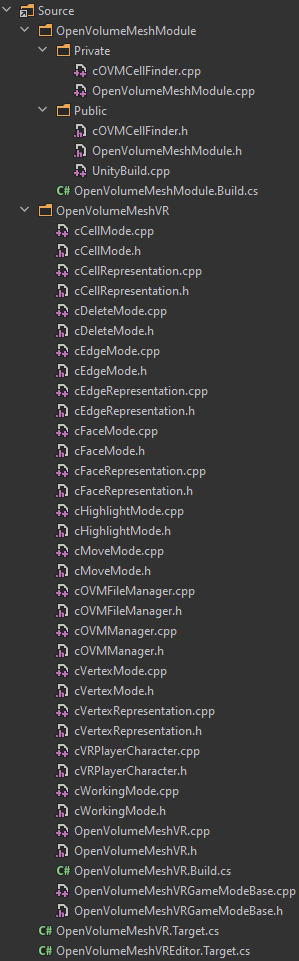
\includegraphics[width=0.28\textwidth]{Project_Structure.png}
				\captionsetup{singlelinecheck = false, justification=justified}
				\caption{Project Structure}
				\label{ProjectStructure}
			\end{figure}
		\end{tabular}
	\end{tabular}

	\section{Functionality for both VR and Mouse-Keyboard Control}
	\startsection
		OpenVolumeMeshVR is able to support both Mouse-Keyboard Control and VR Control. The Mouse-Keyboard Control methods are defined within the AcVRPlayerCharacter class. The VR Control, however, is handled by the engine itself, by binding the position of the head-mounted device with the position of the camera. To make the controllers in VR visible, meshes provided by the Unreal Engine are loaded and displayed if a motion source, also known as the head-mounted device, is tracking. Otherwise, these meshes will not be displayed and only the \textsc{PlacementChaperone}, the replacement for the cursor, is shown. This behavior is controlled within the VRCharacter Blueprint, a blueprint created from the cVRPlayerCharacter C++ File.
		\begin{figure}[H]
			\begin{center}
				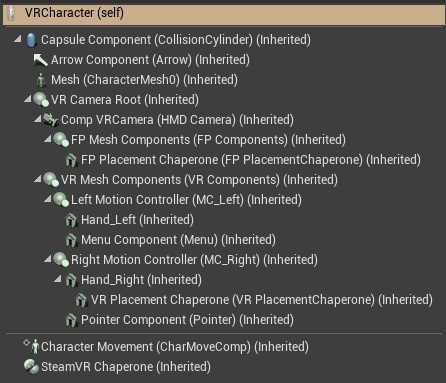
\includegraphics[width=0.35\textwidth]{VRCharacter.png} 
				\caption{Contents of VRCharacter}
				\label{VRCharacterContent}
			\end{center}
		\end{figure}
		\noindent As seen in Figure \ref{VRCharacterContent} It contains a component for VR components and one for Mouse-Keyboard Components. When the VR Character is initialized all of these components will be created. With the help of Unreal Engine's Visual Code, the state of the motion tracking can be queried, and therefore the appropriate components can be shown (Figure \ref{VisualCode}).
		\begin{figure}[H]
			\begin{center}
				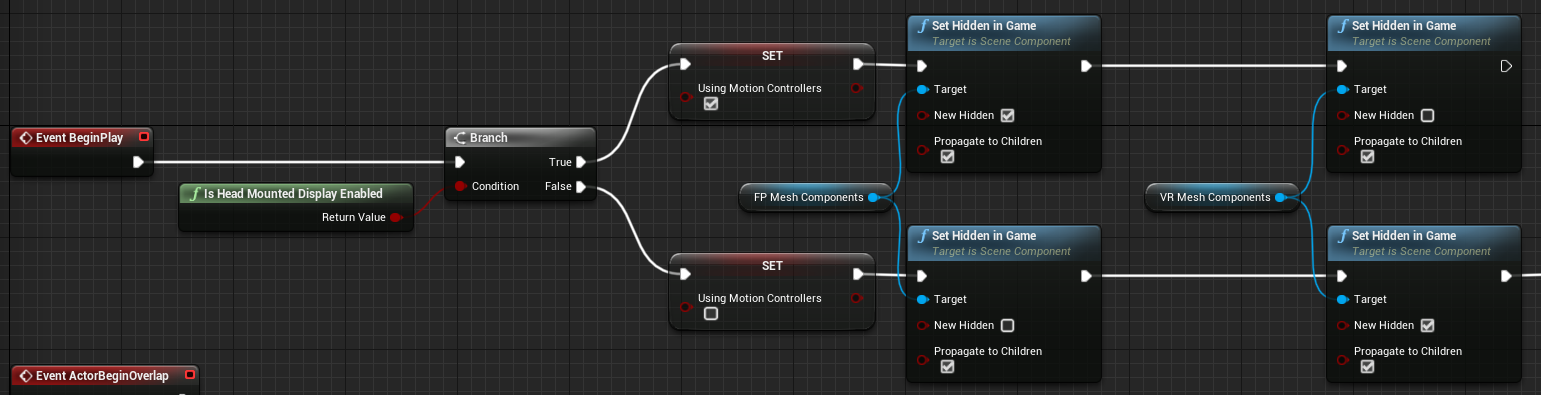
\includegraphics[width=0.85\textwidth]{VisualCode.png} 
				\caption{Visual Code for showing the appropriate components}
				\label{VisualCode}
			\end{center}
		\end{figure}
	\closesection
	
	\section{Representation of Components} \label{ComponentRepresentation}
	\startsection
		The Vertex and Edge Components, the visualization of both these entities, are predefined Assets, Actor Blueprints from C++ Files, within the Unreal Engine. They can be found in UE's content browser in the directory Content/Blueprint/BaseGame/Assets. This approach had the advantage that the functionality of each component, like handling the material or enabling the Tick function in order to move the asset, is integrated by using C++ code whereas the shape can be set in the Blueprint Editor, which is much easier than coding it from anew. Both the vertex and the edge representation are referenced in the VRCharacterBlueprint in which so-called UProperties were added which are class variables that can be set in the Blueprint Editor. This can be seen in Figure \ref{UProperties} in that the UProperties are defined within the code but are set within the Blueprint (red part) therefore not needing any ObjectFinder and can guarantee that the application always spawns the correct component representation. If these should want to be changed either the assets themselves can be altered or new references can be set in the VRCharacter blueprint.
		\begin{figure}[H]
			\begin{center}
				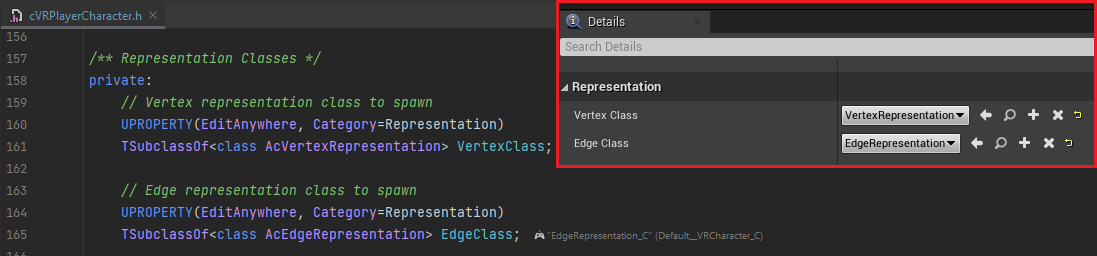
\includegraphics[width=0.95\textwidth]{UProperties.png} 
				\caption{The creation and setting of UProperties}
				\label{UProperties}
			\end{center}
		\end{figure}
		\noindent Because Faces and Cells are created differently - with the use of Unreal Engine's Custom Mesh (Section \ref{CustomMesh}) - there is no blueprint for these assets. \\
		Additionally, different materials were defined such that the highlighting of objects, as well as the indication that the cell finding algorithm has terminated, can be performed. These materials are loaded in the respective constructor of each representation class:
		\begin{minted}{cpp}
static ConstructorHelpers::FObjectFinder<UMaterial>LoadedDefaultMaterial(TEXT("path"));	
		\end{minted}
		This line of code will search for the named material and save it in the LoadedDefaultMaterial struct. With LoadedDefaultMaterial.Succeeded it can be queried whether the loading was successful and with LoadedDefaultMaterial.Object the material instance can be accessed. A similar approach as seen before using UProperties could have been used for the materials as well, but because Faces and Cells do not have any Blueprint associated with them and therefore for these cases the second approach would be inevitable, hence for the sake of consistency this approach was chosen for all components. Consequentially when one wants to change the materials, it has to be done manually or one needs to adjust the path within the code if new materials are imported and are chosen to be used.
	\closesection
	
	\section{Creation of CustomMesh to represent Faces and Cells} \label{CustomMesh}
	\startsection
		Unreal Engine has the option to generate a custom mesh during runtime which will be used as the representation for faces and cells in OpenVolumeMeshVR. A custom mesh is a geometric entity that contains many mesh sections. A mesh section can be understood as a single face from which one can define its vertices and the triangles it is made from. In order to create this kind of entity, first a UProceduralMeshComponent must be instantiated. This class is predefined by the Unreal Engine developers which allow the user to create custom triangle mesh geometry. When creating a face or a cell within OpenVolumeMeshVR an array of vertices, or faces respectively, will be handed over to the function which is responsible for generating the mesh entity. Because a cell is just a scaled-down version of multiple faces, which are therefore corresponding to the individual mesh sections, only the approach for generating a "face mesh" will be clarified. In preparation to create a mesh section first all vertex positions relative to the center of the actual face are added to an array. Then a triangulation is performed in order to create several triangles which will make up the whole face. The current method used in OpenVolumeMeshVR is to create another vertex in the barycenter of the face which does then combines with two adjacent vertices in order to create a triangle. These triangles are saved also in an array similar to how OpenVolumeMesh does, by referring to the index of the vertex in the position array mentioned before. By calling the CreateMeshSection method and handing over the position and triangles array a mesh section is generated by the Unreal Engine.
	\closesection
	
	\section{Integration and Use of OpenVolumeMesh}
	\startsection
		In order to run and build the program on many different platforms also the OpenVolumeMesh framework must be built previously to make the library accessible to the algorithms within the application. In Unreal Engine native C++ libraries can be implemented with the use of modules. A module is a building block in Unreal Engine which contains its Build file. Within this module the required files of the OVM source are included in a UnityBuild file, hence building the OpenVolumeMesh library during the build of the actual application. \\
		This approach has the advantage, unlike by directly linking the OVM library to the project, that the application itself can build on any platform without any need of first building OpenVolumeMesh and searching for the correct library because this does depend on the platform it is used. Also when distributing the project's source code via GitLab the project can be opened within the Unreal Editor and instantly be compiled and used. \\
		If a new entity is spawned into the virtual world a corresponding EntityHandle is added to the PolyhedralMesh data structure. Additionally, an OVM-Property is added to this Handle in order to create a direct difference between it and the actual representation component that was spawned.
	\closesection
	
	\section{Algorithm for Moving Components}
	\startsection
		When moving any kind of component each other component that is adjacent, and therefore directly affected by the movement of it, will also be altered, in either form or position. The main components which are responsible for the movement of all other components are the vertices. If they change their position it will also affect all adjacent edges, faces, and cells. This is implemented this way to mirror the implementation in OVM, because in it also only the vertices have the information about the positions and the other components are referring to the associated vertices. \\
		In order to be able to move vertices the \textit{Tick()} function, which are methods that are called every frame from within the Engine. Within these methods, the \textit{UpdatePositionAndAppearance()} function are called for each other component which is responsible for altering the shape and position of the corresponding representation. It would also have been possible to use the already available \textit{Tick()} methods for the altering process but this led to laggy and stagnant behavior of the application because the user can move the mouse faster than the computer can execute all \textit{Tick()} function and because the rendering function and the \textit{Tick()} functions are executed in their thread, the edges and faces could lag creating an inaccurate representation of the mesh. If everything is called from just a few methods, these inaccuracies are less noticeable or don't occur at all.
	\closesection
		
	\section{Algorithm for Finding Cells} \label{CellMode}
	\startsection
		\subsection{Functionality of the Algorithm}
		\startsubsection
			\begin{tabular}{@{}p{0.65\textwidth}p{0.3\textwidth}@{}}
				When the CellFindingAlgorithm (CFA) is started both class variables are initialized or emptied. One is the \textit{HandleList}, which will contain all the half-faces which make up a valid cell - none if no cell is found. The other one is the \textit{CheckedHandleList}, which will contain all the half-faces that were checked during the search in order to save time and computation power by only needing to check each half-face at most once, are initialized or emptied. The selected half-face, which is the starting point from which the search is initialized, is first checked whether it is already part of a valid cell. If this is the case the search is over because in an OpenVolumeMesh Topology a half-face can only be contained in one cell. Then it is checked whether the half-face is "closed in", meaning that for each edge of it it is checked if it is a boundary of at least one other face (see Figure \ref{ClosedInFace}).
				&
				\begin{figure}[H]
					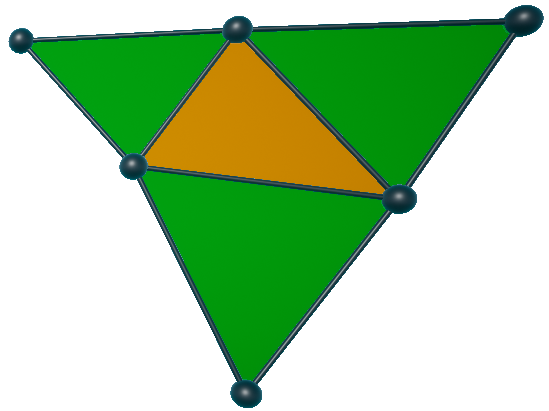
\includegraphics[width=0.275\textwidth]{CellMode_Explanation/ClosedInFace.png}
					\captionsetup{singlelinecheck = false, justification=justified}
					\caption{"Closed-In" Face}
					\label{ClosedInFace}
				\end{figure}
			\end{tabular}
			\noindent If this is the case the half-face is also added to the \textit{HandleList}. The search is then executed as follows:
			\begin{minted}{bash}
Initialize empty CheckedHandleList
Initialize empty HandleList

CFA(HalfFaceHandle):
    add HalfFaceHandle to CheckedHandleList
    if HalfFaceHandle already part of valid cell:
    |   return false
    if HalfFaceHandle closed-in:
    |   add HalfFaceHandle to HandleList
    |   for each half_edge of HalfFaceHandle:
    |   |   int failedCalculations = 0
    |   |   opp_half_edge = opposite of half_edge
    |   |   Initialize empty adjacentHFH
    |   |   save all half-faces adjacent to opp_half_edge in adjacentHFH
    |   |   sort adjacentHFH
    |   |   for each halffacehandle in adjacentHFH:
    |   |   |   if halffacehandle is not in HandleList 
    |   |   |   AND opp_half_edge does not belong to any half-face in HandleList:
    |   |   |   |   if halffacehandle is in CheckedHandleList:
    |   |   |   |   |   failedCalculations++
    |   |   |   |   if CFA(halffacehandle) returns false
    |   |   |   |   |   failedCalculations++
    |   |   if for all halffacehandles in adjacentHFH check failed:
    |   |   |   Remove HalfFaceHandle from HandleList
    |   |   |   return false
    |   return true
    return false
			\end{minted}
			The sorting of the adjacent half-faces is done so the algorithm is faster to find a valid cell if there is any. The sort criterion is the angle between the half-face that was passed to the method and the adjacent half-face. This was chosen because, intuitively, the more acute the angle between two half-faces the more likely it is that this adjacent half-face would lead to a valid cell. The angle is calculated as described in the \href{https://www.w3schools.blog/angle-between-two-planes}{W3Schools-Blog}. \\
			A hands-on example how this algorithm works on a specific mesh can be found in Appendix \ref{appendix:CFAExample}.
		\closesection
		\subsection{Complexity of the Algorithm}
		\startsubsection
			The worst case for this algorithm would be a huge mesh structure in which all of the (half-)faces create one big cell with no smaller inner cells. Therefore the algorithm has to check every single face in order to find that valid cell. Let's assume that there are $N$ faces and on average each face has $m$ neighbors. Because for every half-face the actual recursion method is at most called once there will be $N$ recursion calls. Furthermore, each of the adjacent half-faces must be checked twice, one time for the sorting algorithm and a second time for the actual check. Hence, the complexity of this algorithm lies within $O(N \times 2*m*N) = O(N^2)$.
		\closesection
		\subsection{"Proof" of Termination}
		\startsubsection
			Because all the half-face handles are saved in the CheckedHandleList when they were passed as a parameter to the method and the recursion step is skipped if they are already part of that list, the algorithm will terminate at the very latest if every half-face handle was checked once.
		\closesection
	\closesection
	
	\newpage	
	
	\section{Implementing additional Modes}
	\startsection
		A mode represents the implemented class of a given feature. As concluded in Section \ref{IntuitionStudyConclusion} for each feature that is of use, a different mode should be implemented, i.e. there are four different modes for placing the four different entities vertex, edge, face, and cell. A mode like the edge or the face mode is considered to have a continuous mode because after the first vertex is placed the behavior of the code must be changed in order to create an edge or even a whole face. \\
		When implementing a mode it must be of type \textbf{AcWorkingMode}. AcWorkingMode is an abstract Actor, which behaves like an interface because Unreal Engine does not give a developer the option to use an actual interface for this usage. The code within the header class of the new file (suppose the new mode is called NewMode) will look like the following:
		\begin{minted}{cpp}
  // cNewMode.h file		

  #include "cWorkingMode.h"		
		
  class OPENVOLUMEMESHVR_API AcNewMode : public AcWorkingMode
  {
      GENERATED_BODY()
				
      // Declaration of variables and methods
  }
		\end{minted}
		The following 4 methods are necessary for each mode and must therefore be overridden (more information can be get from the documentation of the code):
		\begin{minted}{cpp}
  // What happens if the left-mouse button/right B-trigger is clicked
  virtual void AcceptSelection(class AcVRPlayerCharacter * cActor, ...) override;

  // If the WorkingMode contains a continuous mode this method will handle the
  // "Undo" function if the mode is terminated or switched while being actively used
  // (i.e. deleting all newly spawned entities)
  virtual void ForceUndo(class AcVRPlayerCharacter* cActor) override;

  // Returns true if the mode is in the continuous working mode (which will also
  // indicated at the top of the HUD) and false otherwise
  virtual bool IsInContinuousWorkingMode() override;

  // The name of the mode that should be displayed in the HUD
  virtual FString ToString() override;
		\end{minted}
		To also be accessible during the game the \textit{VRPlayerCharacter} must include this new mode and the new mode must be instantiated when the corresponding number key is pressed. In the cVRPlayerCharacter.cpp there are already predefined methods called ChangeModeX, where X is the number corresponding to the button pressed. The code within this method must be changed accordingly:
		\begin{minted}{cpp}
  void AcVRPlayerCharacter::ChangeModeX()
  {
      ResetMode();
      CurrentMode = NewObject<AcNewMode>();
  }	
		\end{minted}
		Furthermore, in the blueprint editor of Unreal Engine for HUD display which is shown during the game, a fitting image should be placed on the corresponding canvas to ensure usability and information delivery to the actual user. The logic for displaying this picture in the top left corner, when that mode was chosen, also has to be implemented in the visual code of the HUD display.
	\closesection
	
	
\chapter{Conclusion}	
	The goal of this bachelor thesis - creating an application for generating and modifying OpenVolumeMesh meshes was achieved. However, due to the circumstances, the VirtualReality part of this application is not as mature as it was intended to be and the mouse-keyboard control became the primary way of control. Also, many different modes that were proposed in the beginning to be implemented were either discarded due to not being as relevant, like the coloring of different components, or due to the lack of time. Nevertheless, with the program, it is possible to create OVM meshes fast and even a CellFindingAlgorithm, which was not part of the proposal and became a major part of this bachelor thesis during the development of OVMVR, was integrated in order to make the cell generation handier.


\chapter{Future Work}
	During the development of OpenVolumeMeshVR, a few different ideas popped up which can be implemented in a future version of it.
	\paragraph{Snapping Mode Extention} \hfill \\
	Future versions could add the entity-snap functionality, like a vertex in the middle of an edge or face, or implement a degree snapping for generating edges or faces. Additionally, length snapping could also be an option.
	\paragraph{Coloring of Entities} \hfill \\
	By coloring single vertices, edges, faces, or even cells certain attributes of the mesh can be highlighted. A color gradient along edges and faces can also be implemented if the adjacent vertices are differing in color.
	\paragraph{Quality Metric of OVM} \hfill \\
	OpenVolumeMesh provides many different quality metrics for example for cells which can be integrated by highlighting the particular part of the mesh.
	\paragraph{Placing cameras for different perspectives} \hfill \\
	In Unreal Engine, it is possible to spawn cameras that will open in a new window in order to be able to view the mesh from different perspectives at the same time. This will greatly enhance the possibilities for showcases of a mesh.
	\paragraph{Multiplayer} \hfill \\
	When in the Unreal Engine Editor itself it is possible to use OpenVolumeMeshVR in a multiplayer environment. This possibility is not given if the application is built and also within the editor it is not working reasonably well. It may be a great experience to work with others and generate a mesh together.
	\paragraph{Increase the Limit of Entities} \hfill \\
	As of now, the soft limit cap of entities of OpenVolumeMeshVR is approximately 5'000. By using culling or changing the render distance within the UnrealEngine or by altering the representations, for example via a level of detail (LOD) approach, this limit could be greatly increased.
	\paragraph{Implement Undo and Redo function} \hfill \\
	While a user is creating a mesh errors can happen. Therefore it might be a good idea to have an undo and redo function within the application to quickly correct these errors.	
	\paragraph{Improvements for the Triangulation Algorithm for the Generation of Mesh Sections} \hfill \\
	For the creation of mesh sections, one must first define the triangles from which it is made of. Currently, an additional vertex is placed in the middle of the face and all the other vertices next to each other are connected in sequence with it in order to create the triangles. For better results, this triangulation algorithm can be changed and adjusted.

\newpage
\addcontentsline{toc}{chapter}{Literature}
\bibliography{literature}

\appendix
	
\chapter{Intuition Study: Evaluation Sheet} \label{appendix:questionnaire}
	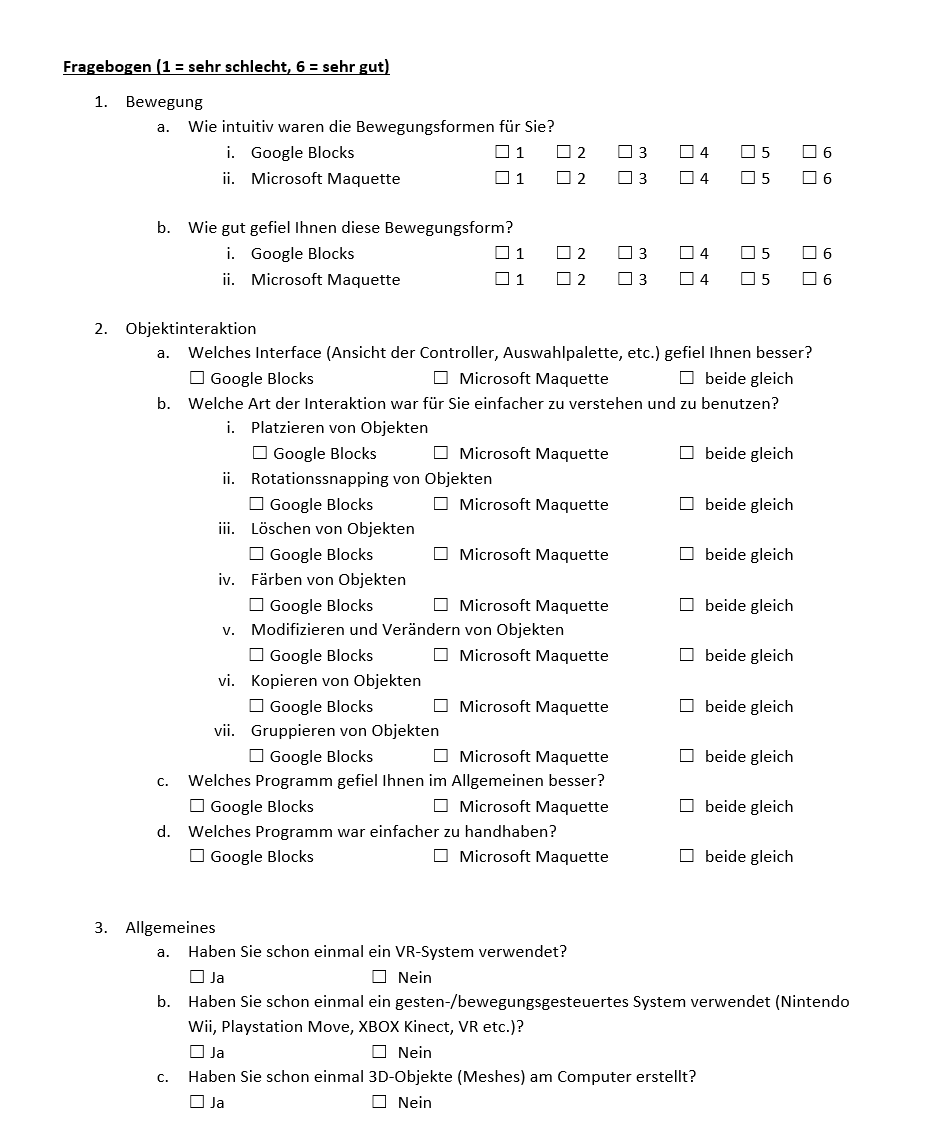
\includegraphics[width=0.85\textwidth]{Intuitiontest_Questionnaire.png}
	
\chapter{CellFinding Algorithm Example} \label{appendix:CFAExample}
	To visualize the procedure of the CellFinding algorithm, the following mesh is used as an example (most of the highlighting is not shown in the editor at runtime; only the result is marked in red). The whole algorithm is working with half-faces but because OVMVR is only able to display the faces and not the individual half-faces this additional information must be mentally added:
	\begin{figure}[H]
		\centering
		\begin{subfigure}[H]{3in}
			\centering
			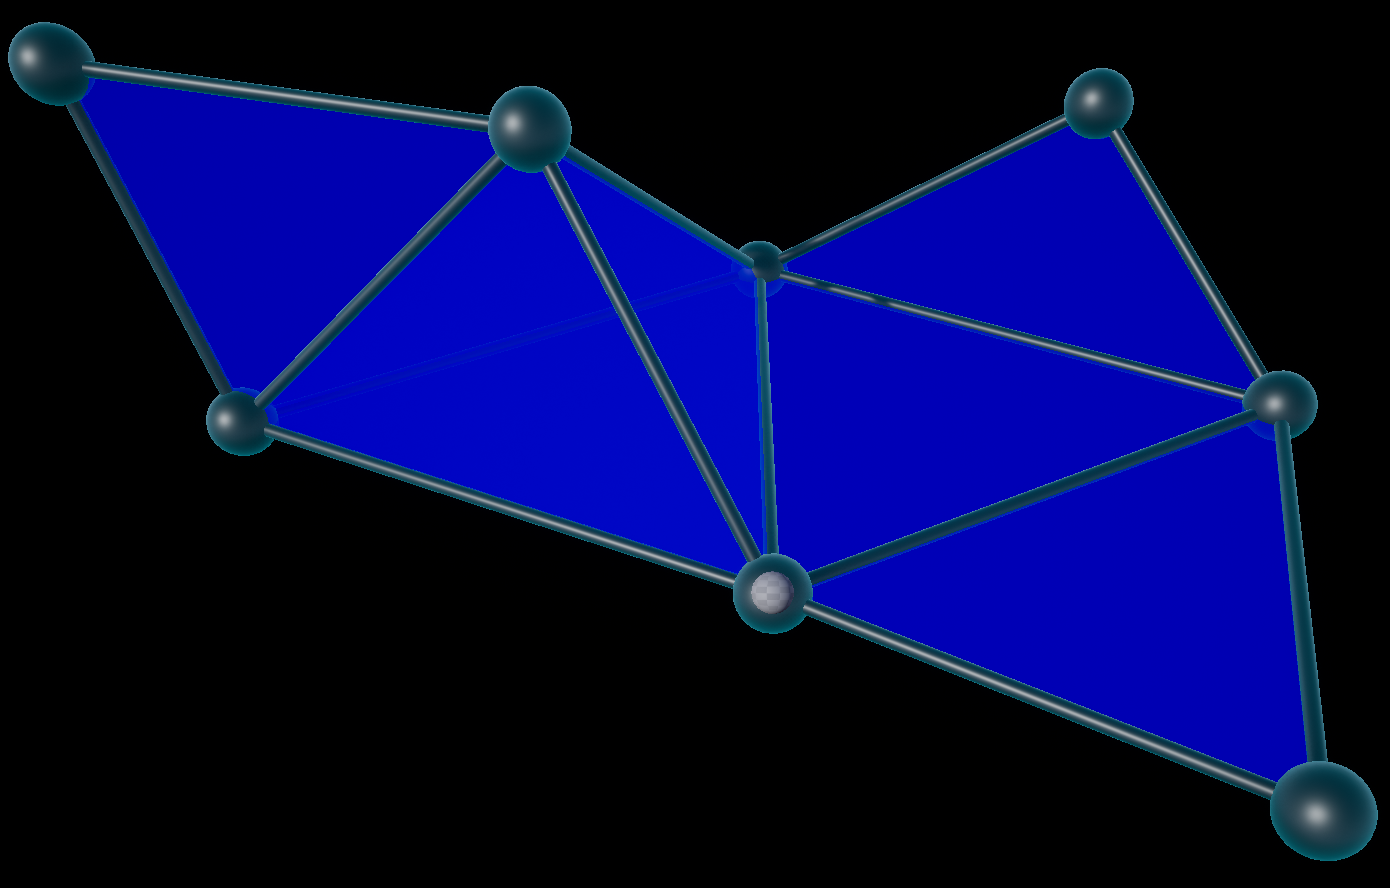
\includegraphics[scale=0.175]{CellMode_Explanation/InitialState.png}
			\label{pic:picB.1.a}
		\end{subfigure}
		\quad
		\begin{subfigure}[H]{3in}
			\centering
			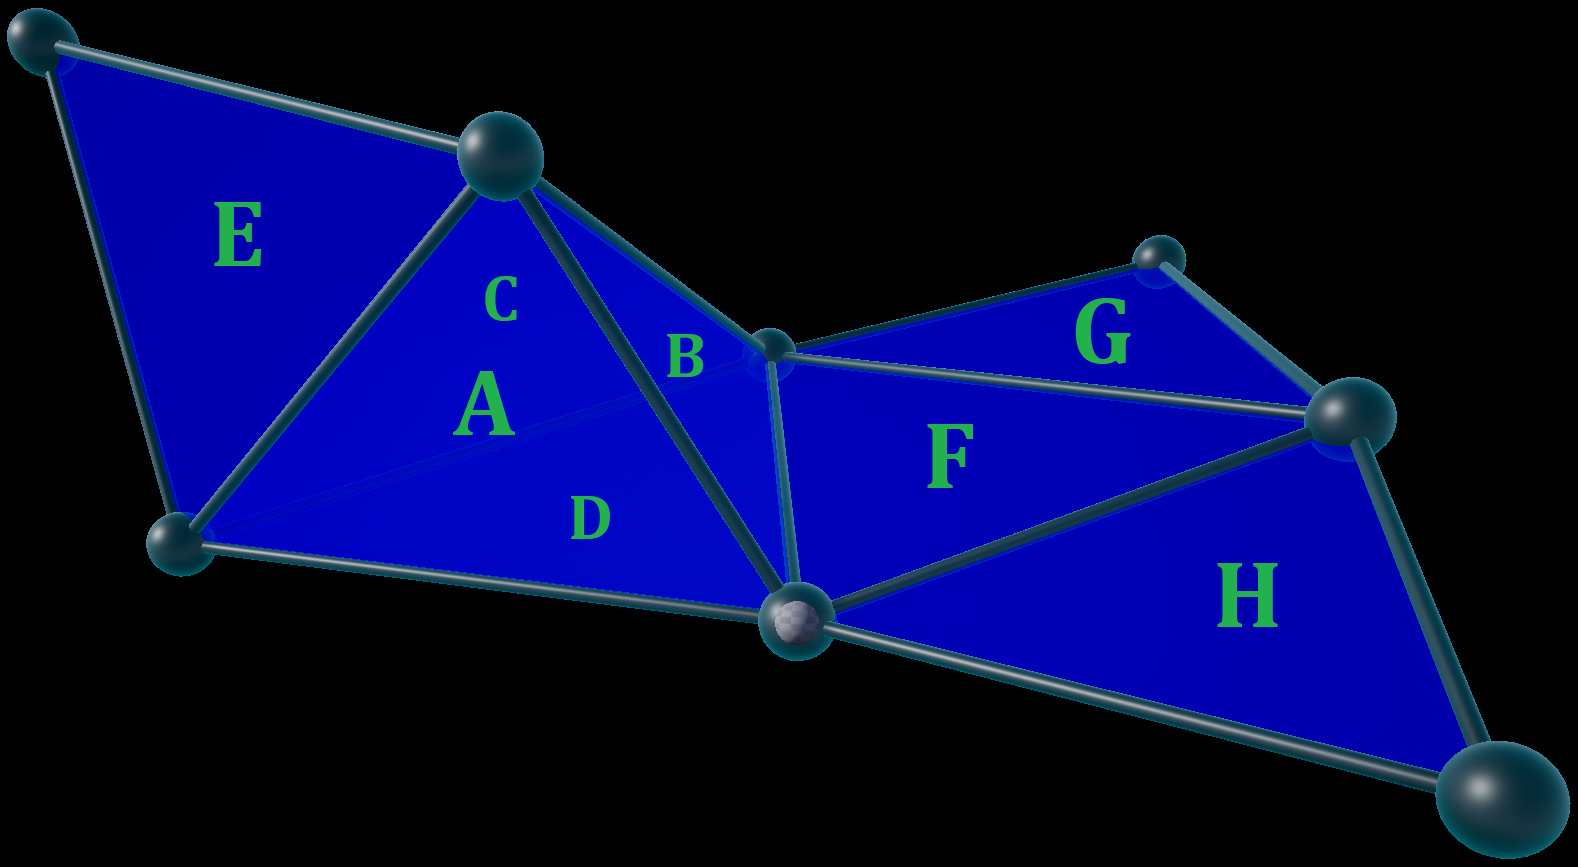
\includegraphics[scale=0.175]{CellMode_Explanation/InitialState_labeled.png}
			\label{pic:picB.1.b}
		\end{subfigure}
		\caption{Initial Mesh}
		\label{pic:picB.1}
	\end{figure}
	\noindent The user wants to create a cell by selecting the half-face of face \textbf{A}, which is facing away from the viewer.
	\begin{center}
		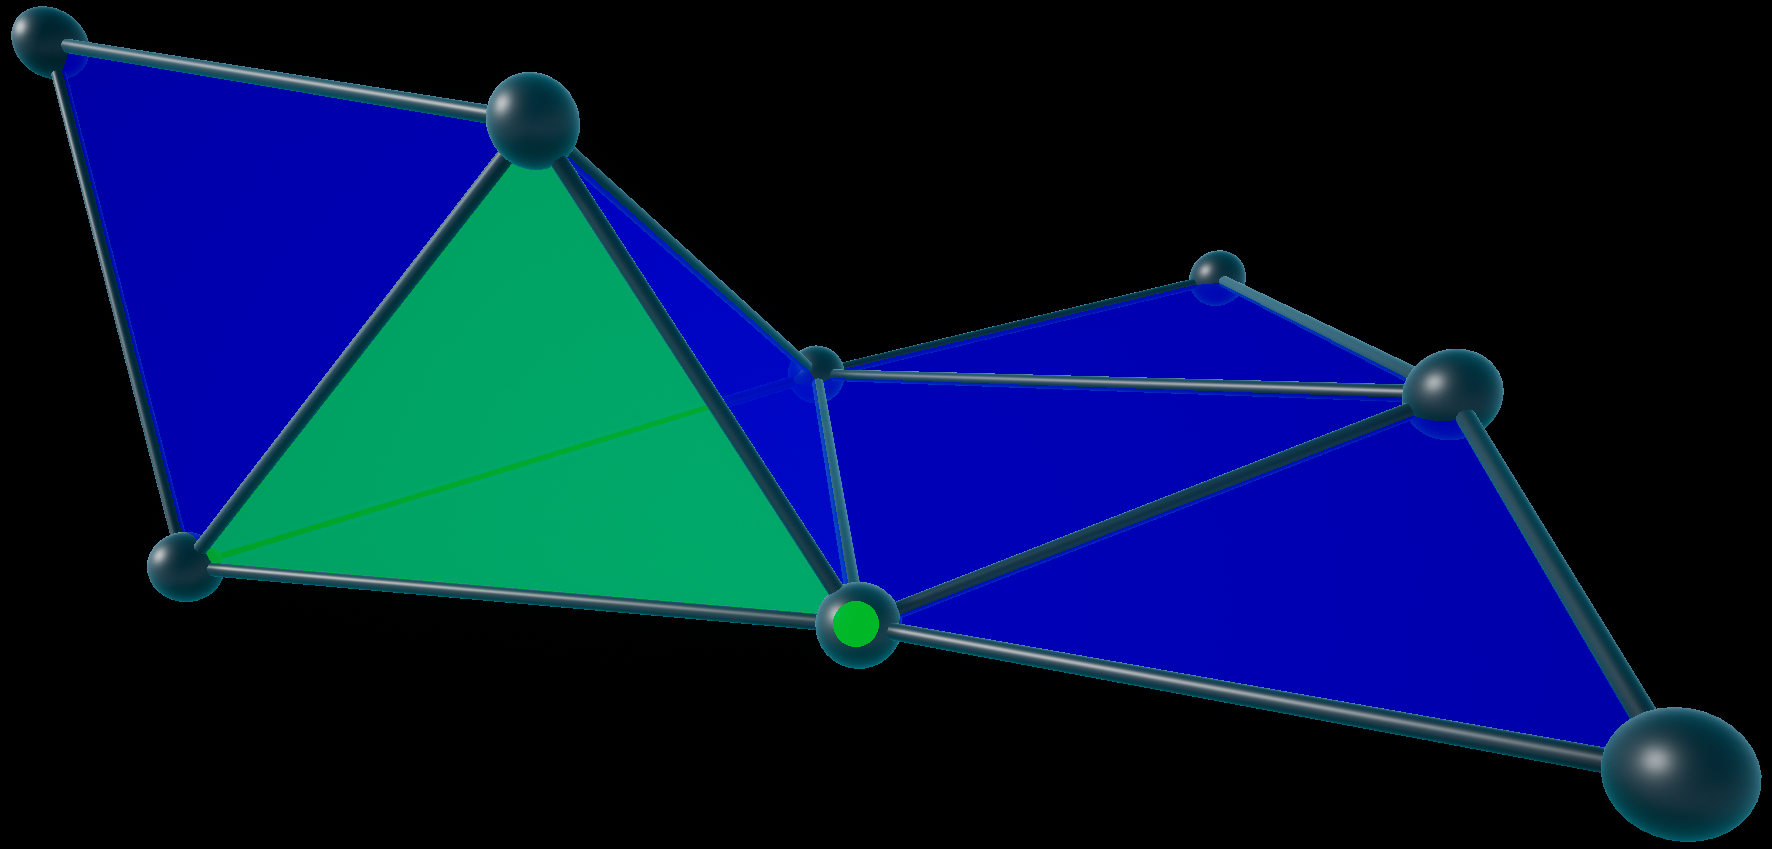
\includegraphics[scale=0.15]{CellMode_Explanation/SelectedHalfFace.png}
		\captionof{figure}{Selected Face}
		\label{pic:picB.2}
	\end{center}
	First, the algorithm will check whether there is already a valid cell containing this half-face and whether the half-face is "closed-in". As the selected half-face passes these checks the adjacent edges are iteratively checked whether they have half-faces that lead to a valid cell or not.
	\begin{center}
		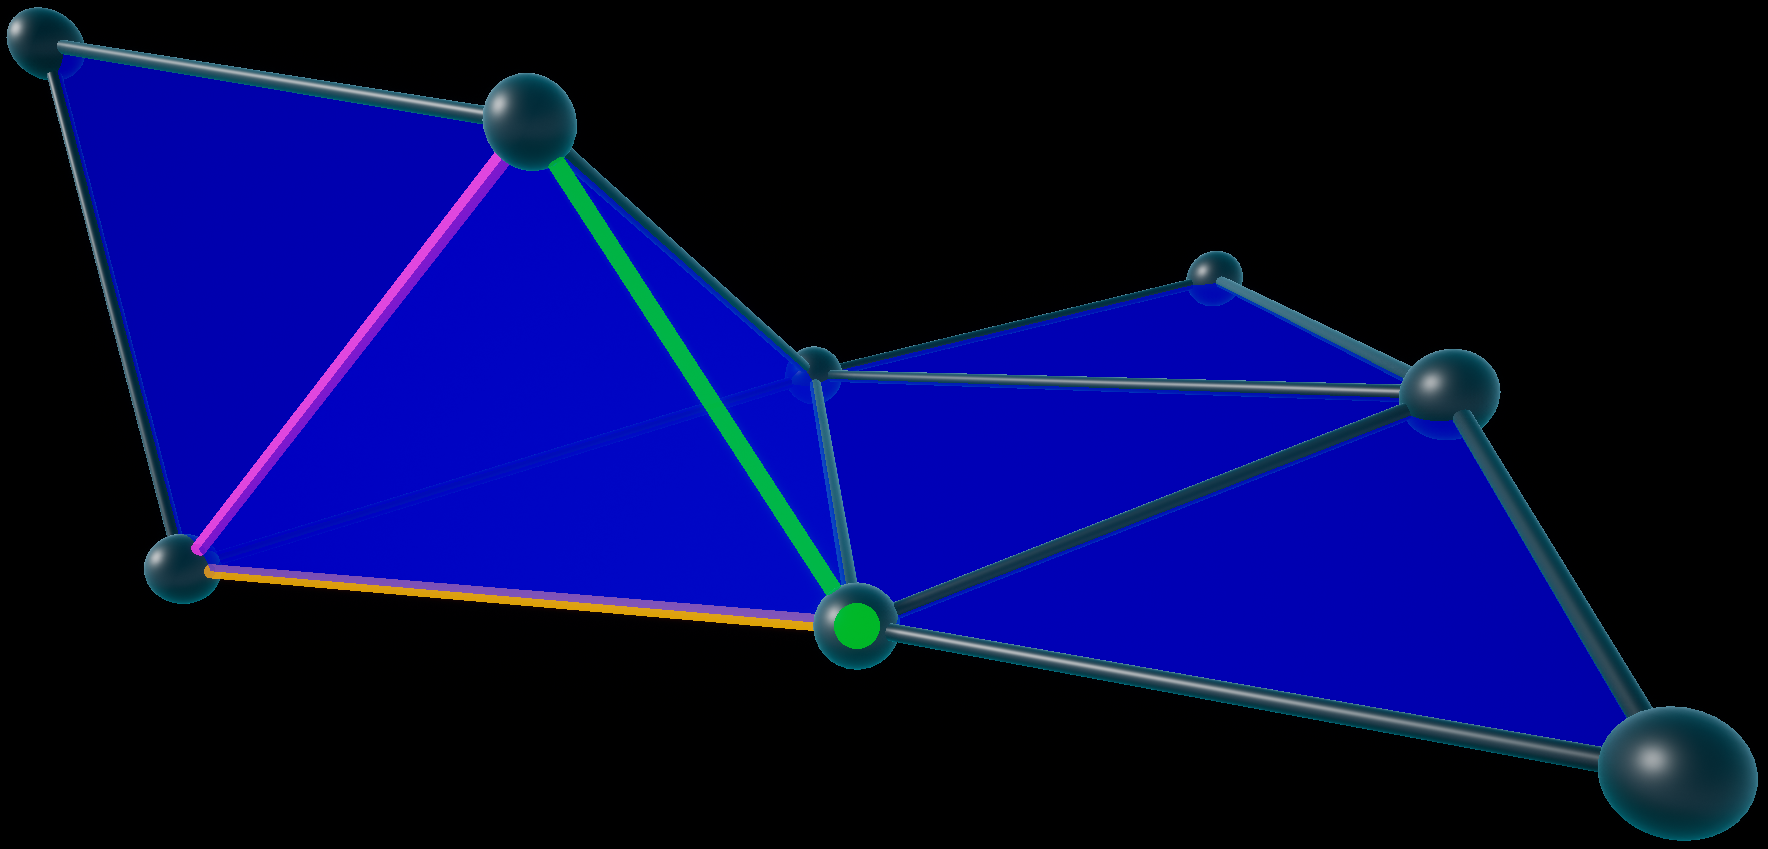
\includegraphics[scale=0.15]{CellMode_Explanation/AdjacentEdges.png}
		\captionof{figure}{Adjacent Edges}
		\label{pic:picB.3}
	\end{center}
	Because it is somewhat random which edge is chosen first for checking, here it will be assumed that the pink edge is the first in the list. The associated half-faces of this edge are then saved into a list and the angle to the previous half-face is calculated.
	\begin{center}
		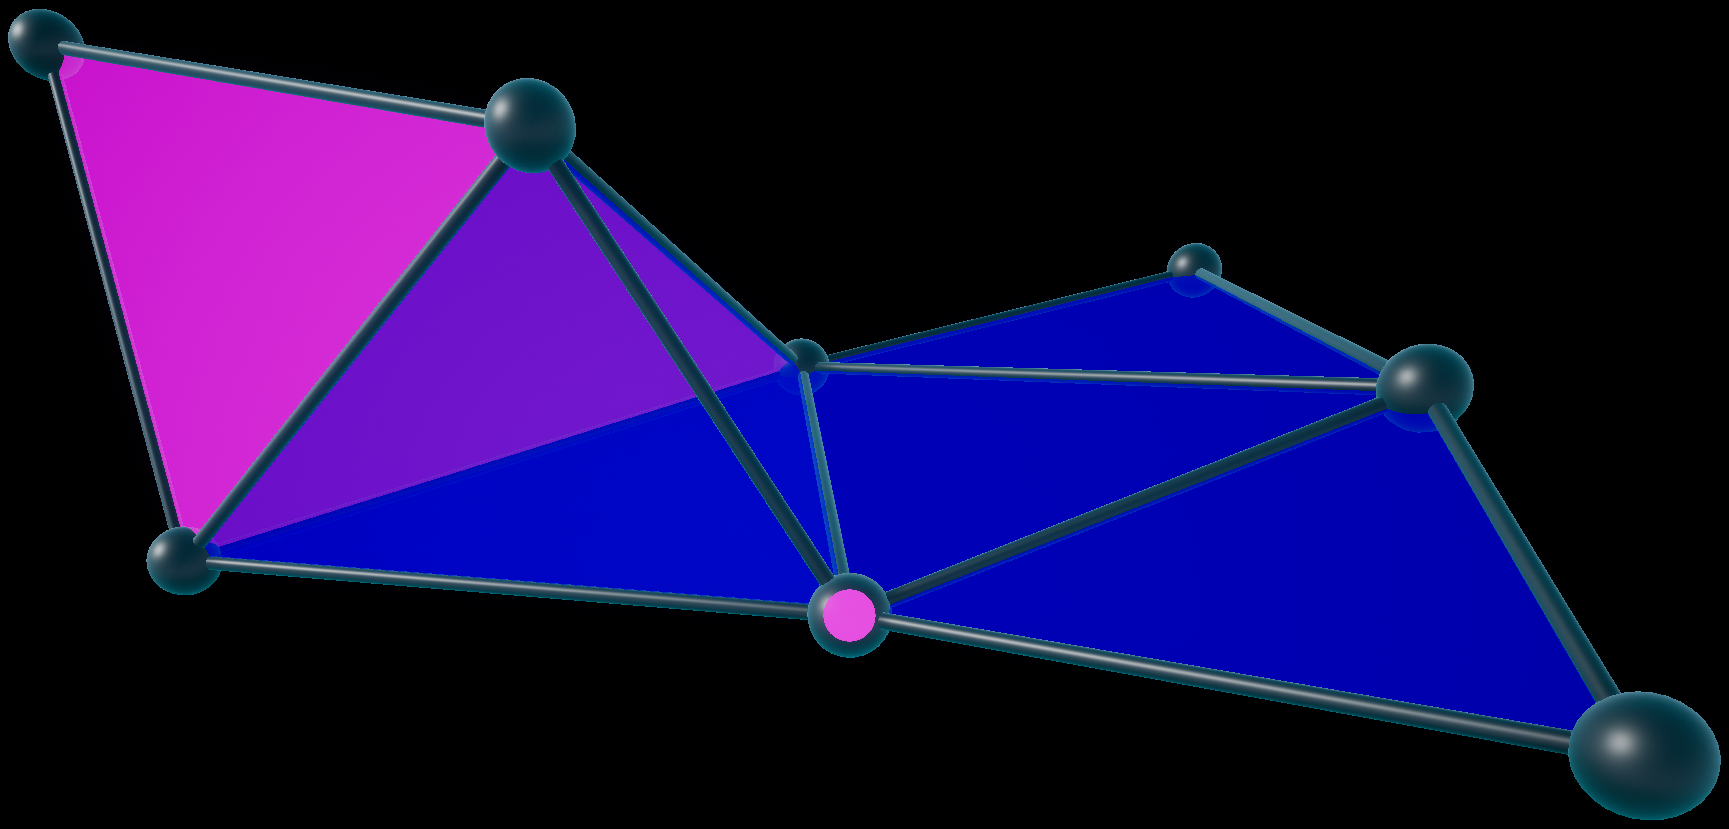
\includegraphics[scale=0.15]{CellMode_Explanation/StepOne.png}
		\captionof{figure}{Adjacent Half-Faces}
		\label{pic:picB.4}
	\end{center}
	The half-face \textbf{C}, that is part of the tetrahedron, has a more acute angle to the front half-face than the one that points out to the left (half-face \textbf{E}). Therefore it is chosen to be checked first and will be passed to the recursion algorithm. As it is also passing all the checks of not being part of a valid cell and being "closed-in" it will be added to the HandleList, which will therefore contain the following two half-faces (\textbf{A} and \textbf{C}):
	\begin{center}
		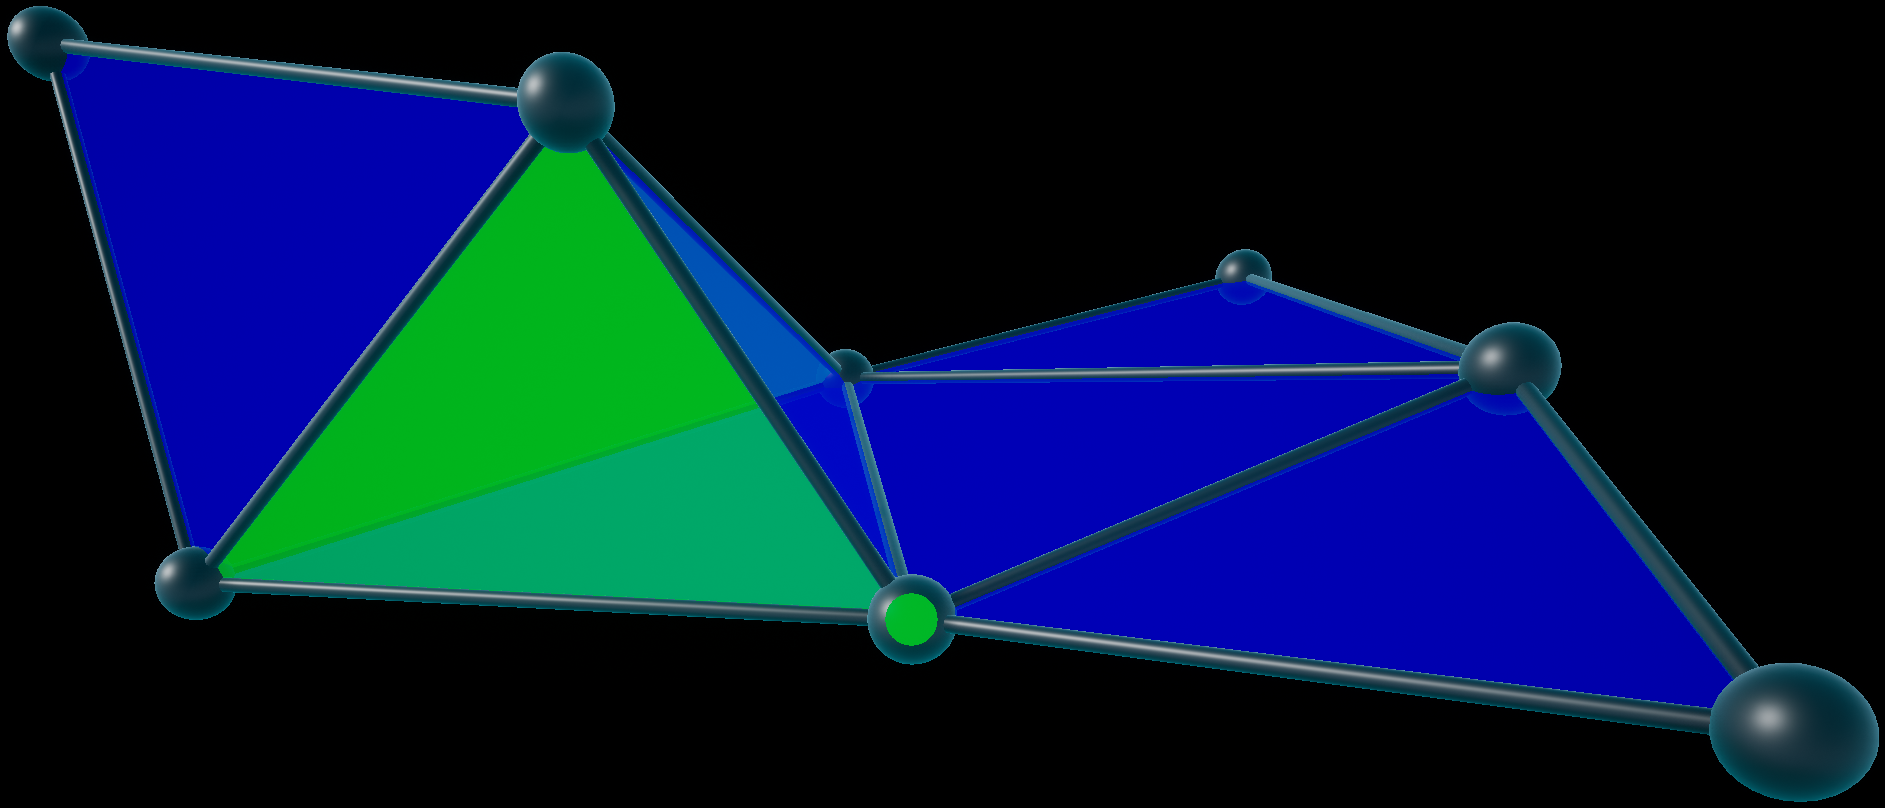
\includegraphics[scale=0.15]{CellMode_Explanation/HandleList1.png}
		\captionof{figure}{Contents of HandleList}
		\label{pic:picB.5}
	\end{center}
	Because the algorithm is doing the checks for half-face \textbf{C}, the next half-face that is checked will be edge \textbf{B} - again it is assumed that the edge connecting both faces \textbf{C} and \textbf{B} is first in the list.
	\begin{center}
		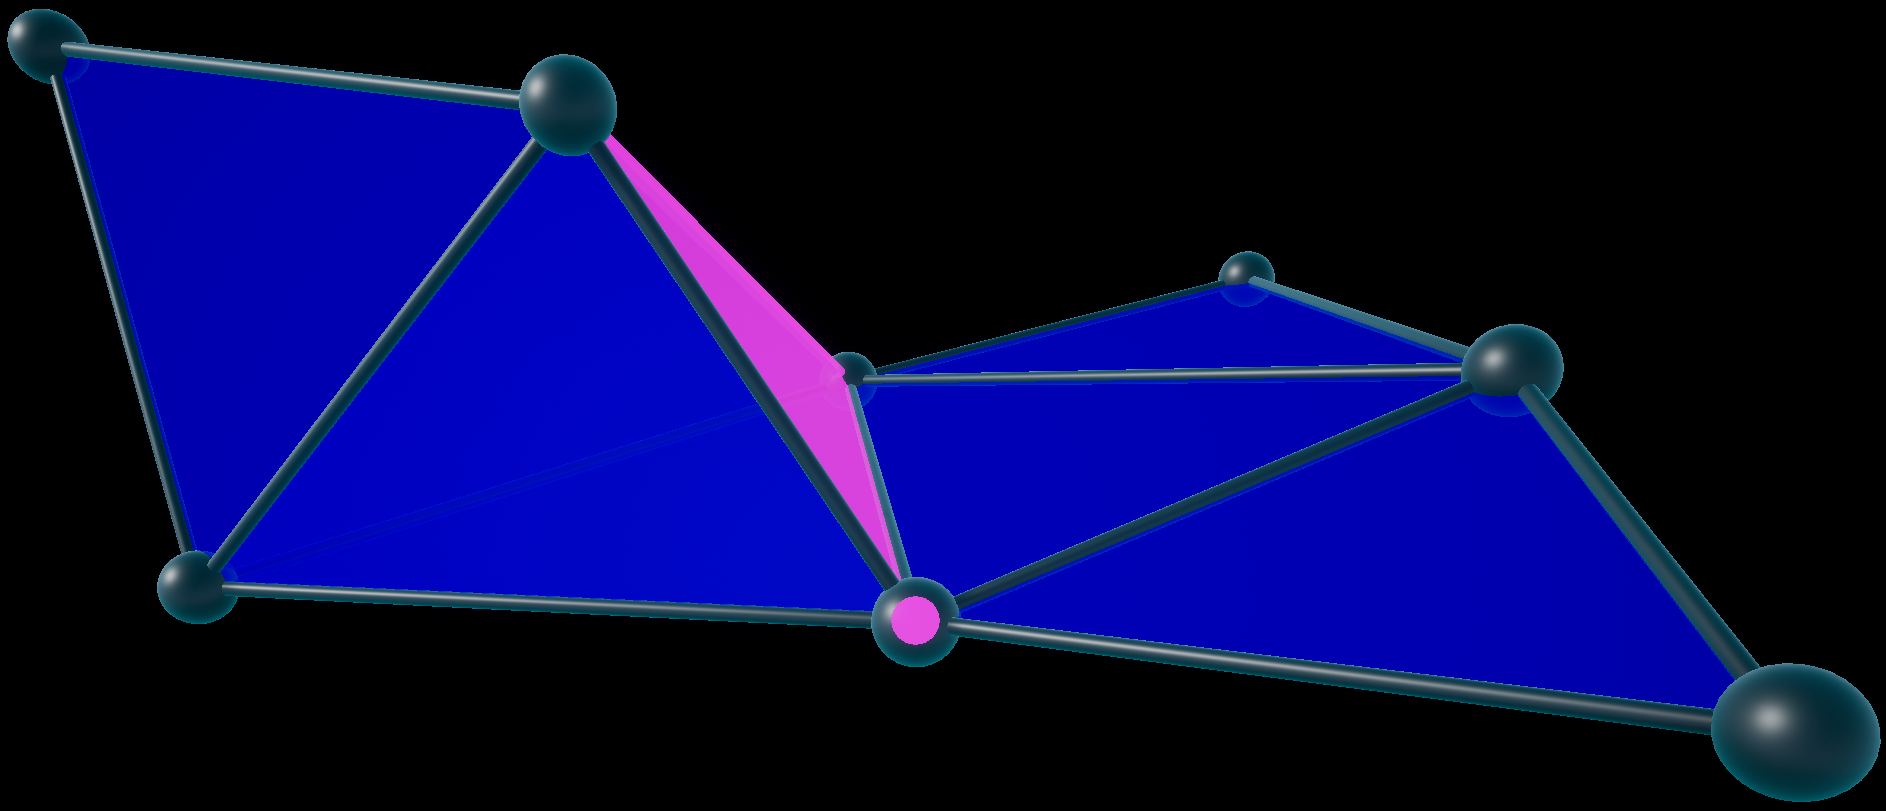
\includegraphics[scale=0.15]{CellMode_Explanation/StepTwo.png}
		\captionof{figure}{Adjacent Half-Face}
		\label{pic:picB.6}
	\end{center}
	As this half-face \textbf{B} is also passing the checks it wil be added to the HandleList:
	\begin{center}
		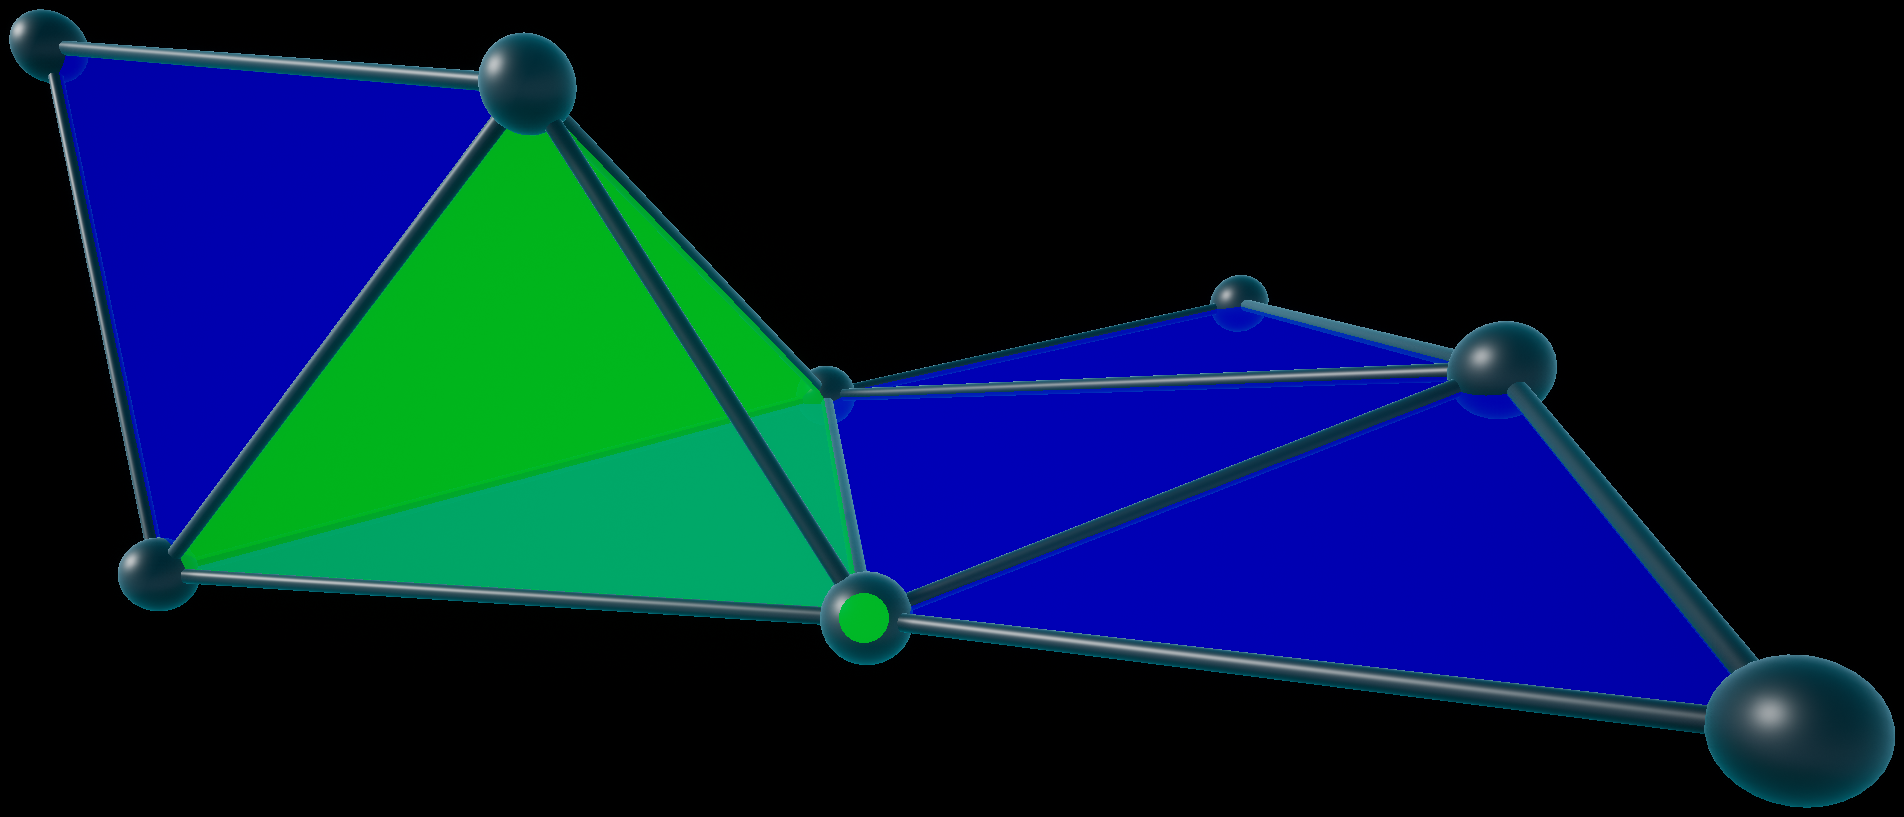
\includegraphics[scale=0.15]{CellMode_Explanation/HandleList2.png}
		\captionof{figure}{Contents of HandleList}
		\label{pic:picB.5}
	\end{center}
	The next step is to consider the bottom edge of half-face \textbf{B} which is connecting to half-faces \textbf{D} and \textbf{F}.
	\begin{center}
		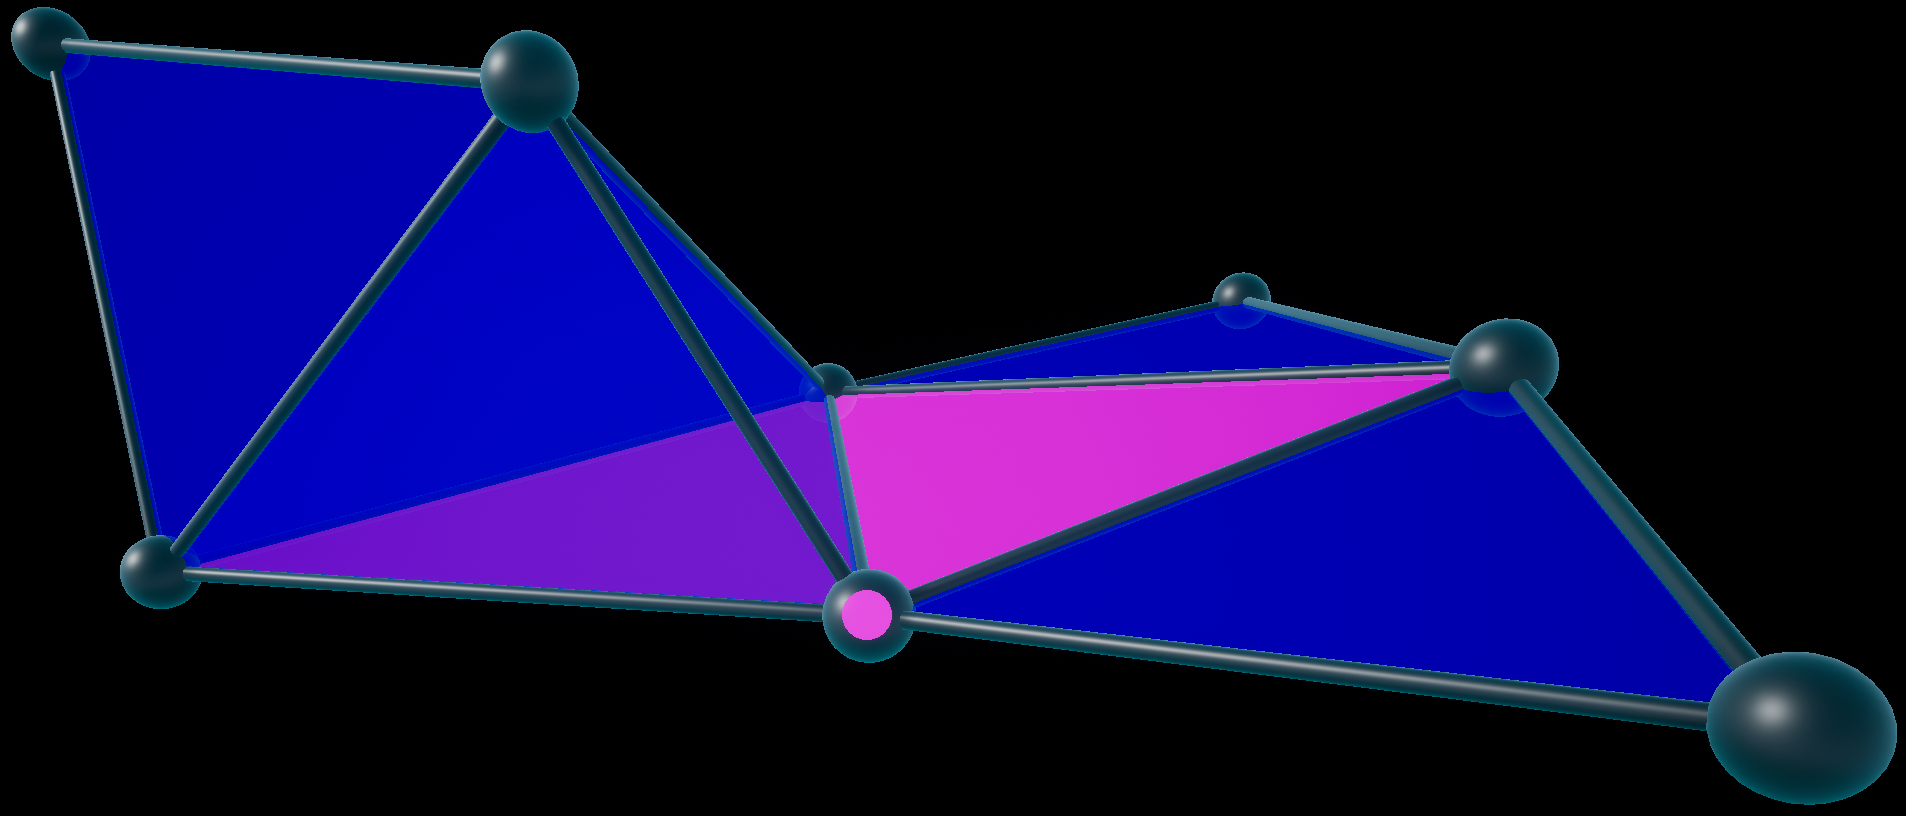
\includegraphics[scale=0.15]{CellMode_Explanation/StepThree.png}
		\captionof{figure}{Adjacent Half-Faces}
		\label{pic:picB.6}
	\end{center}
	 As \textbf{D} has a much sharper angle than \textbf{F} towards \textbf{B}, it will be checked first and will be added to the HandleList.
	 \begin{center}
		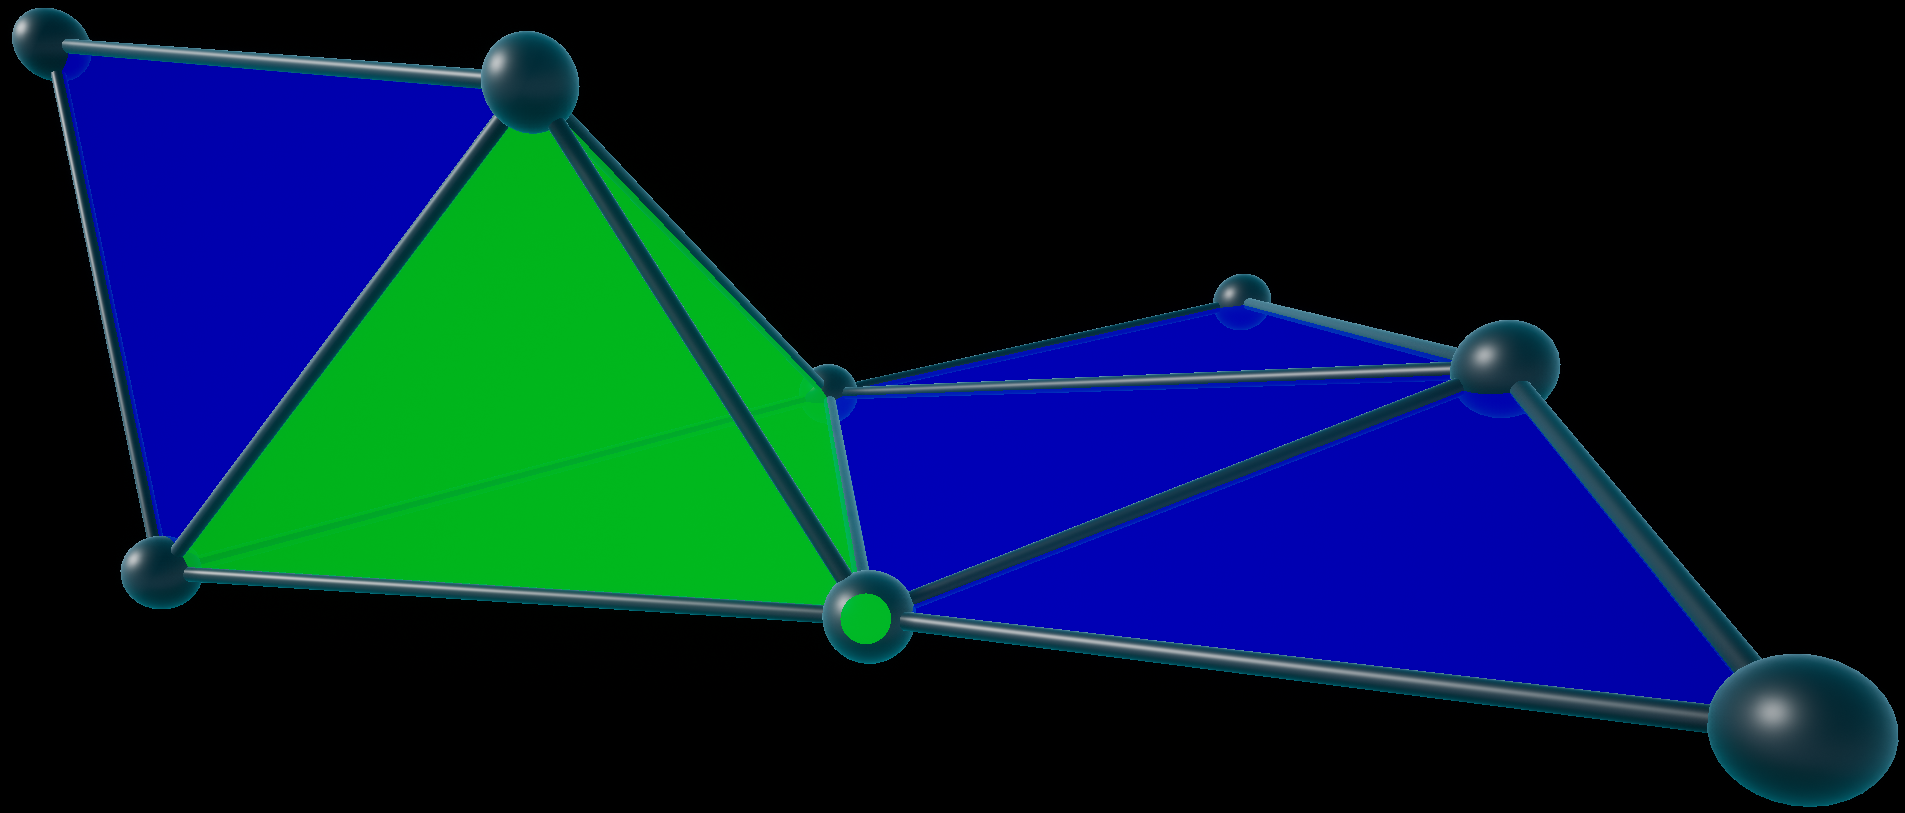
\includegraphics[scale=0.15]{CellMode_Explanation/HandleList3.png}
		\captionof{figure}{Contents of HandleList}
		\label{pic:picB.5}
	\end{center}
	Now that each of the adjacent half-faces of \textbf{D} is already in the HandleList each of those edges will \textit{return true}, therefore also half-face \textbf{D} is returning true. Next would be the check of half-face \textbf{F} because it is the second adjacent half-face of \textbf{B}. As this edge already contains a half-face, namely \textbf{D}, that is contained within the HandleList, this check is skipped and half-face \textbf{B} will also \textit{return true}. The same is true for half-face \textbf{C}. Half-face \textbf{E} is again skipped because the edge connecting it with half-face \textbf{A} already has a half-face that is contained within the HandleList. In the end half-face \textbf{A} will \textit{return true}, highlighting the found cell \textbf{A B C D}.
\end{document}
